\setchapterpreamble[u]{\margintoc}
\glsresetall % reset glossary
\chapter{Enriching the classic TTO formulation with advanced mechanical constraints}

Chapter 3 highlighted some inherent limitations of the truss modeling and the conventional optimization formulation of \gls{tto}. These limitations include the minimum slenderness problem and the absence of local buckling and kinematic compatibility constraints. The primary objective of this chapter is to propose a comprehensive formulation capable of addressing these shortcomings. As we will observe, the resulting formulation, if solved in its original form, tends to yield solutions characterized by numerous active and intersecting bars. To mitigate this, we propose a two-step optimization algorithm that offers a means to reduce the solution complexity. Additionally, we introduce a heuristic designed to reduce the influence of the starting point within this two-step optimization algorithm. \marginnote{Part of the content presented in this chapter has been published \todo{finish}.}

In \secref{sec:04_constr}, we detail and model the various mechanical constraints applied in the context of \gls{tto}. Subsequently, in \secref{sec:04_formulation_and_algo}, a comprehensive formulation is presented along with an accompanying optimization algorithm. Through the utilization of this optimization algorithm, we are able to maintain control over the complexity of the design. Finally, in \secref{sec:04_numerical_app}, we put the proposed formulation to the test, applying it to various 2D and 3D test cases sourced from the literature, as well as novel cases. The objective is to assess its capabilities and numerical performance.

\section{Advanced mechanical constraints} \label{sec:04_constr}
This section aims to introduce additional mechanical constraints that will be utilized in this study, to reduce the need for post-processing at the end of the optimization process, just before the manufacturing phase begins. We begin by addressing the issue of minimum slenderness, a side constraint that is imposed on the cross-sectional area of the active members to guarantee that the solution adheres to the truss modeling. Subsequently, we address the local buckling constraints, a critical failure mode observed in ultra-light truss structures. Particular attention is devoted to examining the stability of nodes within what are known as compressive chains. The combination of local buckling and nodal stability, a phenomenon known in the literature as topological buckling, is discussed. Furthermore, as we want our formulation to be as versatile as possible, we explore the extension of these constraints to accommodate multi-load cases. A challenge arises from the fact that the resulting structures are frequently statically indeterminate. To address this, we introduce an additional mechanical constraint known as "kinematic compatibility" to ensure that the predicted force field aligns with the displacements of the structure.

\begin{table*}
    \small
    \centering
    \resizebox{\columnwidth}{!}{%
    \begin{tabular}{
        V{5cm}
        V{2.5cm}
        V{1.7cm}
        V{2.5cm}
        V{2.2cm}
        V{2.5cm}
        V{2cm}}
        \toprule
    Authors &
      Stress &
      Local Buckling &
      Topological buckling &
      Kinematic compatibility &
      Multi-load cases &
      Minimum slenderness
       \\ \midrule
    Dorn et al. (1964)  \cite{dorn_automatic_1964}                & x &-&-&-&-&-\\
    Hemp (1973)  \cite{hemp_optimum_1973}                       & x &-&-&-& x &-\\
    Reinschmidt et al.   (1974) \cite{reinschmidt_applications_1974}         & x & x &-& $\sim$ &-&-\\
    Kirsch (1980) \cite{kirsch_optimal_1980}                       & x &-&-& x &-&-\\
    Oberndorfer et al. (1996)   \cite{oberndorfer_two_1996}        & x & x &-&-&-&-\\
    Silva Smith (1997)  \cite{silva_smith_topology_1997}                & x & x & $\sim$ &-& x &-\\
    Achtziger (1999a, 1999b) \cite{achtziger_local_1999,achtziger_local_1999b}            & x & x & x &-& x &-\\
    Stolpe (2004)   \cite{stolpe_global_2004}                    & x & x &-& x & x &-\\
    Pritchard et al. (2005)  \cite{pritchard_plastic_2005}           & x &-&-&-& x &-\\
    Tyas et al. (2006)   \cite{tyas_practical_2006}               & x & x & x &-& x &-\\
    Descamps et al. (2014)  \cite{descamps_nominal_2014}            & x & x & x &-& x &-\\
    Schwarz et al. (2018) \cite{schwarz_efficient_2018}              & x & x &-&-&-&-\\
    Cai et al. (2022)  \cite{cai_topology_2022}                 & x & x & x &-&-&-\\
    Present work                        & x & x & x &x&x&x\\ \bottomrule
    \end{tabular}}
    \caption{Non-exhaustive list of the existing research in Truss Topology Optimization (TTO) with their corresponding scientific contributions.}
    \label{tab:04_literature}
\end{table*}

In \tabref{tab:04_literature}, we provide an overview of historical and contemporary research in the field of \gls{tto}, along with their respective scientific contributions. This serves to highlight the necessity for a more comprehensive formulation that incorporates these mechanical constraints, reducing the gap between the optimized design and the actual manufactured structure.
    
\subsection{Minimum slenderness constraints}
As previously discussed in \secref{sec:03_applications}, the \gls{tto} method shows numerous limitations due to its reliance on the truss model. Therefore, the resulting structures may not be acceptable if the model falls outside the bounds of this idealization. To better study this limit, as outlined in \secref{sec:03_applications}, we introduced a metric called bar slenderness, which is defined as follows:
\begin{equation}
    \lambda = \frac{\ell}{R_{\mathrm{g}}},
\end{equation}
where $R_{\mathrm{g}}$ represents the gyration radius of the cross-sectional area, defined as $R_{\mathrm{g}} = \sqrt{I/a_i}$.
The primary objective of this section is to introduce an upper limit constraint on the cross-sectional area design variable. This constraint prevents a bar from exceeding the bounds of its idealized model, thereby enhancing the optimization process's robustness.

Remembering that for a circular cross-section $I = \pi r_i^4/4$, we can write
\begin{equation}
    R_{\mathrm{g},i} = \frac{r_i}{2}.
\end{equation}
The minimum slenderness limit constraints are then stated as:
\begin{equation} \label{eq:04_slend_constraints}
    a_i \leq \frac{4 \pi \ell_i^2}{\lambda_{\text{max}}}, \quad \forall i \in [1,\ldots, N_{\text{el}}]
    \tag{$\vect{g}_{\text{slend}}$}
\end{equation}
for a fixed $\lambda_{\text{max}}$. In this thesis we set $\lambda_{\text{max}}=15$.

\subsection{Local and topological buckling constraints}
Adding local buckling constraints to the optimization formulation is fundamental, as ultralight truss structures are often dominated by this mode of failure \sidecite{sigmund_non-optimality_2016}. By imposing local buckling constraints over a \gls{tto} problem (where the lower bound for the members' cross-sectional areas is 0), the optimization domain becomes disjointed \sidecite{cheng_aspects_1995}. The solution is to be searched inside a degenerate space of the design space of the optimization, known in the literature as singular optimum \sidecite{guo_new_2001}. Stolpe \sidecite{stolpe_note_2003} showed how using the \gls{sand} formulation with local buckling and kinematic compatibility constraints, it is possible to find well-optimized structures without the use of relaxation techniques. The authors, however, point out how the solution is still very sensitive to the initialization point of the \gls{nlp} formulation. The local buckling constraints $\vect{g}_{\text{buck}}$ are stated using Euler's critical load formula as:
\begin{equation}
    q_i  + \frac{s_i a_i^2}{\ell_i^2} \geq 0 \quad \forall i \in [1,\ldots, N_{\text{el}}],
    \tag{$\vect{g}_{\text{buck}}$}
    \label{eq:04_buck}
\end{equation}
where $s_i$ is a parameter dependent on the member material and section topology as follows:
\begin{equation}
    s_i=\pi^2 E \beta_i.
    \label{eq:04_s}
\end{equation}
$\beta_i=I_i/a^2_i$ is a positive constant dependent on the moment of inertia and the section of the $i$-th bar, and $E$ is Young's modulus of the material. Assuming that the shape of the cross-section is identical over the whole structure and is independent of $a$, it follows that  $\beta_i = \beta$ and $s_i = s, \; \forall i \in [1,\ldots, N_{\text{el}}]$.

Direct application of the local buckling constraint \eqrefnotext{eq:04_buck} in the optimization formulation tends to create "chains" of unstable compressive members \sidecite{bendsoe_optimization_1995, zhou_difficulties_1996, rozvany_difficulties_1996}. This problem is known in the literature as topological buckling \sidecite{achtziger_local_1999}, as the definition of the compressive chains is a function of the topology of the structure, and is one of the elements of the nodal stability of the structure. Additional forms of structure instability, such as global buckling \sidecite{ben-tal_optimal_2000,kocvara_modelling_2002, neves_generalized_1995, ferrari_topology_2021} or the use of lateral perturbing forces to obtain nodal stability \sidecite{tyas_practical_2006,mela_resolving_2014} have been studied in the literature. However, since they are beyond the scope of this work, they will not be discussed further.

\begin{figure}
    \centering
    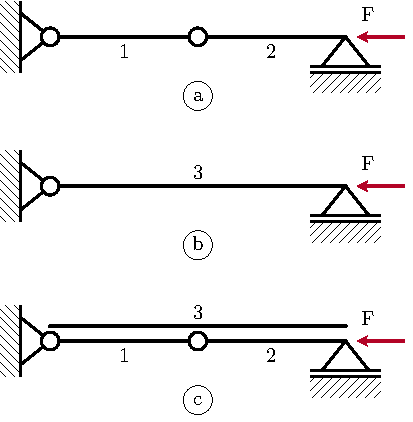
\includegraphics{figures/04_TTO_improvements/01_3_bars_chain/3_bars_chain.pdf}
    \caption{The three ground structures loaded in compression are used to highlight the topological buckling problem in \gls{tto}. (a) Two-bar ground structure loaded in compression; (b) single bar ground structure; (c) overlap of the $a$ and $b$ ground structures.}
    \label{fig:04_chain_buck}
\end{figure}

To illustrate the topological buckling phenomenon, we consider the case shown in \figref{fig:04_chain_buck}a. It consists of a ground structure with $M=3$ nodes and $N_{\text{el}}=2$ bars with length $\ell_1=\ell_2=\ell$, and a compressive load of magnitude $F$ applied at the right-hand side node. For this trivial structure, we can state that $q_1=q_2=F$ and thus $a_1=a_2=a$. We suppose here that the allowables of the material are such that the local buckling (and not the stress) is the most limiting failure criterion for the bars. Assuming that the shape of the section is equal, the local buckling constraints are written as:
\begin{equation}
    q_i\geq -\frac{s a^2}{\ell^2}, \quad i\in[1,2].
    \label{eq:04_chain_1}
\end{equation}
However, the structure is unstable because the vertical force equilibrium equation evaluated on the central hinge is satisfied only in an ideal case where no structural imperfections are taken into account.

If the hinge between bars 1 and 2 is deleted, we obtain the structure pictured in \figref{fig:04_chain_buck}b with $\ell_3=2\ell$. The local buckling constraints for bar 3 are thus:
\begin{equation}
    q_3\geq -\frac{s a_3^2}{(2\ell)^2}.
    \label{eq:04_chain_2}
\end{equation}

Combining \eqsref{eq:04_chain_1}, \eqrefnotext{eq:04_chain_2} and observing that $q_1=q_2=q_3=F$, it is now trivial to demonstrate that $a_3=2a$. Constraint \eqrefnotext{eq:04_chain_2} leads, then, to more voluminous structures compared to constraint \eqrefnotext{eq:04_chain_1}. For that reason, even if we consider the ground structure given in \figref{fig:04_chain_buck}c composed by the superposition of the ground structures in \figref{fig:04_chain_buck}a and \figref{fig:04_chain_buck}b, the optimization with a uniform initialization tends to converge to the solution $\vect{a}^*=[a,a,0]$, unstable but lighter than the physical solution $\vect{a}_p^*=[0,0,2a]$. 

The easiest way to get rid of the instability of the compressive chains is to post-process the optimized structure and remove the unstable hinges between the compressive bars. Doing that, the local buckling constraints are not satisfied anymore as the effective buckling length has increased. It is, then, necessary to calculate the section of the new compressive bars to comply with the newly introduced buckling constraints. As extensively shown by Achtziger \sidecite{achtziger_local_1999b}, this post-processing phase leads to structures that are less optimal compared to the ones we could obtain if we take into account the topological buckling in the optimization in the first place.

For that reason, Achtziger proposes an update strategy to modify the length used to evaluate the critical buckling force of \eqrefnotext{eq:04_buck} as follows:
\begin{equation}
    \ell^*_i(\vect{a}):= 
    \begin{cases}
        \ell_i & \text { if } i \notin \mathcal{C}_{l,r}(\vect{a}) \\
        \sum \ell_{r} \;|\; r \in \mathcal{C}_{l,r}(\vect{a})  & \text { otherwise,}
    \end{cases}
    \label{eq:04_chain_len}
\end{equation}
where $r$ represents the $r$-th bar of the $l$-th compression chain of the structure. The topology-dependent set $\mathcal{C}_{l,r}(\vect{a})$ is defined as the set of $r$ member indexes of the $l$-th buckling chain. As internal forces on buckling chains are constant, only the buckling length of the first member of the chain ($\ell^*_i(\vect{a}) \text{ with } i \in \mathcal{C}_{l,1}(\vect{a})$) is modified. Additionally, we add the following side constraints on the other members of the $l$-th chain to ensure feasibility:
\begin{equation}
    a_{r}\geq a_{r=1} \quad \; r \in \mathcal{C}_{l,r}(\vect{a}), \; \forall r \neq 1.
    \label{eq:04_side_cons_chain}
\end{equation}

\subsection{Kinematic compatibility constraints}
To optimize test cases that result in statically indeterminate structures, such as structures loaded with multiple load cases or imposed symmetries, we add an additional mechanical constraint called kinematic compatibility \sidecite{kirsch_optimal_1989, rozvany_layout_1995}. Compatibility can be imposed as a nonlinear constraint in the optimization formulation \sidecite{kirsch_optimal_1980}, or can be taken into account by prestressing the initial structure \sidecite{kirsch_effect_1989}.

The kinematic compatibility constraints restrict the displacement field $\vect{U} = [U_1, \ldots,U_{N_{\text{dof}}}]^T$ in such a way that strains $\varepsilon_i$ and internal stresses $\sigma_i$ comply with Hooke's law $\sigma_i = E_i \varepsilon_i$ with $i \in [1,\ldots, N_{\text{el}}]$. Recalling that in a truss the relationship between nodal displacements and member deformations is $\vect{b}^T_i \vect{U} = \ell_i \varepsilon_i$ with $\vect{b}$ as the $i$-th column of the $\matr{B}$ matrix, we can formulate the kinematic compatibility constraints $\vect{g}_{\textrm{comp}}$ as:
\begin{equation}
\label{eq:04_compatib}
     q_i - \frac{a_i E_i}{\ell_i} \vect{b}_i^T\vect{U}  = 0  \quad \forall i \in [1,\ldots, N_{\text{el}}].
     \tag{$\vect{g}_{\textrm{comp}}$}
\end{equation}
Kinematic compatibility constraints are non-linear as the design variable $\vect{q}$ is dependent on $\vect{a}$ and $\vect{U}$.


\section{Optimization formulation and solving strategy} \label{sec:04_formulation_and_algo}
\label{sec:04_method}
In this section, we propose an innovative \gls{tto} formulation developed specifically to minimize the mass of 3D ultralight truss structures, taking into account maximum stress, topological buckling, kinematic compatibility, and minimum slenderness constraints. Combining Formulation \eqrefnotext{eq:03_optim_original} with \eqsref{eq:04_buck} \eqrefnotext{eq:04_slend_constraints}, \eqrefnotext{eq:04_chain_len}, \eqrefnotext{eq:04_side_cons_chain}, and \eqrefnotext{eq:04_compatib}, Formulation $\mathbb{P}_1$ is stated in terms of members' cross-sectional area $\vect{a}$, member forces $\vect{q}$ and nodal displacements $\vect{U}$ as follows:
\begin{equation}
    \begin{aligned}
    \underset{\vect{U}^0, \dots, \vect{U}^{N_p}}{\min_{\vect{a}, \vect{q}^0, \dots, \vect{q}^{N_p},}}   && V &= \vect{\ell}^{T}\vect{a}\\
    \textrm{s.t.}   && \matr{B}\vect{q}^p &= \vect{f}^p && \forall p \in [0,\dots,N_p]\\
    && \vect{q}^p &= \frac{\vect{a}E}{\vect{\ell}}\vect{b}^T\vect{U}^p && \forall p \in [0,\dots,N_p] \\
    && \vect{q}^p &\geq -\frac{s\vect{a}^2}{\vect{\ell}^{*2}} && \forall p \in [0,\dots,N_p] \\
    && -\sigma_\text{c}\vect{a} &\leq \vect{q}^p \leq \sigma_\text{t}\vect{a} && \forall p \in [0,\dots,N_p] \\
    && a_{r}&\geq a_{r=1} && r \in \mathcal{C}_{l,r}(\vect{a}) \\
    && 0 &\leq \vect{a} \leq \frac{4 \pi \vect{\ell}^2}{\lambda_{\text{max}}}. \\
    \end{aligned}
    \tag{$\mathbb{P}_1$}
    \label{eq:04_optim_complete}
\end{equation}
The formulation has been extended to multiple load cases given by $N_p$ external loads vector $\vect{f}^0, \dots, \vect{f}^{N_p}$ and the resulting internal forces $\vect{q} = [\vect{q}^0,\dots, \vect{q}^{N_p}]$ and displacements $\vect{U} = [\vect{U}^0,\dots, \vect{U}^{N_p}]$. This proposed formulation expands the multiple load cases formulation of Achtziger \sidecite{achtziger_local_1999} with kinematic compatibility constraints, permitting the correct evaluation of the mechanical state of statically indeterminate structures.

The formulation follows the \gls{sand} approach \sidecite{sankaranarayanan_truss_1994}, where, in addition to the members' cross-sectional area $\vect{a}$, the member forces $\vect{q}$ and the structure displacements $\vect{U}$ are used as state variables. One of the advantages of \gls{sand} approach is that the state variables are independent of each other and, thus, the sensitivity calculation of the constraints functions is usually simpler and leads to sparse partial derivatives. Additionally, compared to \gls{nand} formulations, the problem stays well-posed even if the cross-sectional area goes to 0. As the linear system $\matr{K}\vect{U}=\vect{f}$ is never explicitly solved during the optimization, it is not necessary to impose a lower bound on the members' cross-sectional area $\vect{a}$ to avoid a singular stiffness matrix. The last important advantage is that thanks to $\vect{U}$ being design variables, it is trivial to add bound constraints on the nodal displacements of the structure if needed.

\subsection{Optimization strategy} \label{sec:04_2step_opt}
Formulation \eqrefnotext{eq:04_optim_complete} presents multiple constraints and design variables for every physical bar of the ground structure. The quantity of constraints creates a highly non-linear design space and it proved to be hard for the optimizer to bring to zero the value of the cross-sectional areas. If a \gls{nlp} optimizer is directly used on Formulation \eqrefnotext{eq:04_optim_complete}, the resulting structure will be composed of a multitude of intersecting bars. The optimizer is, thus, working like it is performing sizing optimization instead of topology optimization. 

Inspired by the early works by Reinschmidt \sidecite{reinschmidt_applications_1974}, we propose a novel two-step optimization strategy in which a first optimization solving a relaxed formulation is used to find a good starting point for the second optimization, solving the full Formulation \eqrefnotext{eq:04_optim_complete}. Doing that way, the first optimization explores extensively the relaxed and more regular design space and finds simpler structures, while the second optimization refines the solution imposing additional mechanical constraints. The complete solving strategy is graphically presented in \figref{fig:04_sol_alg}.

In the first step, Problem \eqrefnotext{eq:04_optim_complete} is relaxed: kinematic compatibility constraints are omitted. We call this relaxed Problem $\mathbb{P}_2$. Problem $\mathbb{P}_2$ is solved using a \gls{slp} method by iteratively linearizing the local buckling constraints. A heuristic strategy called Reinitialization is iteratively used to reduce the influence of the starting point $\vect{a}_0$. The resulting structure described by the design variables vector $\vect{\tilde{x}}^*$ is then post-processed, removing the members whose optimized area is below a fixed cross-sectional area threshold value. The structures generated by solving the relaxed Problem $\mathbb{P}_2$ proved to be simpler \ie fewer active members compared to directly solving \eqrefnotext{eq:04_optim_complete} with a \gls{nlp} optimizer. If the solution is not statically indeterminate the optimization is completed as the kinematic compatibility constraints \eqrefnotext{eq:04_compatib} are automatically satisfied and, thus, used to evaluate the optimal displacements.

Otherwise, a second step is needed. Firstly, the ground structure of the problem is simplified, removing all the members that do not appear in the solution of the relaxed Problem $\mathbb{P}_2$ \ie avoiding the reintroduction of members discarded by the \gls{slp} step. Then, the kinematic compatibility and the exact local buckling constraints are restored, and Problem \eqrefnotext{eq:04_optim_complete} is solved in its original form on the simplified ground structure using a \gls{nlp} optimizer. The initial values for the cross-sectional areas are the solution $\vect{\tilde{x}}^*$ of Problem $\mathbb{P}_2$.

\begin{figure*}
    \centering
    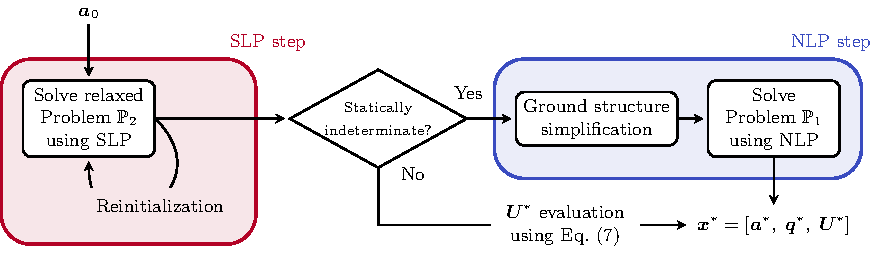
\includegraphics[width=\linewidth]{figures/04_TTO_improvements/02_solution_algo/sol_algo.pdf}
    \caption{Flowchart of the two-step optimization strategy used to solve Problem \eqrefnotext{eq:04_optim_complete}.}
    \label{fig:04_sol_alg}
\end{figure*}

\subsection{First step: SLP optimization}
The first step of the proposed optimization strategy is here described in detail. The relaxed Problem $\mathbb{P}_2$ obtained by omitting \eqrefnotext{eq:04_compatib} and the displacements $\vect{U}$ in Formulation \eqrefnotext{eq:04_optim_complete} is stated as:
\begin{equation}
    \begin{aligned}
    \min_{\vect{a}, \vect{q}^0, \dots, \vect{q}^P}  && V &= \vect{\ell}^{T}\vect{a}\\
    \textrm{s.t.}   && \matr{B}\vect{q}^p &= \vect{f}^p && \forall p \in [0,\dots,N_p]\\
    && \vect{q}^p &\geq -\frac{s\vect{a}^2}{\vect{\ell^{*2}}} && \forall p \in [0,\dots,N_p] \\
    && -\sigma_\text{c}\vect{a} &\leq \vect{q}^p \leq \sigma_\text{t}\vect{a} && \forall p \in [0,\dots,N_p] \\
    && a_{r}&\geq a_{r=1} && r \in \mathcal{C}_{l,r}(\vect{a}) \\
    && 0 &\leq \vect{a} \leq \frac{4 \pi \vect{\ell}^2}{\lambda_{\text{max}}}. \\
    \end{aligned}
    \tag{$\mathbb{P}_2$}
    \label{eq:04_optim_no_constr}
\end{equation}

Since the objective function and all of its constraints are linear, except for the buckling constraint, this problem is solved by iteratively linearizing the non-linear buckling constraints and using a \gls{slp} algorithm. Following the work of \sidecite{schwarz_efficient_2018}, the Euler's critical load is iteratively updated using a first-order Taylor expansion for every $i$ member with cross-sectional area $a_{i}^k$ at the iteration $k$ in the neighborhood of the point $\vect{P}_{k}$ (see \figref{fig:04_SLP}):
\begin{equation}
    \tilde{q}_{i,k}^{\text{cr}} = q_{i,k}^{\text{cr}}(a_{i}^k) + (a_{i}^{k+1} - a_{i}^k)\left.\derfrac{q_{i,k}^{\text{cr}}(a_{i}^k)}{a}\right\rvert_{a=a_{i}^k}
\end{equation}
where $a_{i}^{k+1}$ represent the design variable of the \gls{slp} at the current iteration and $q^{\text{cr}}_{i,k}(a_{i}^k) = -s ({a_{i}^k})^2/\ell^{*2}_i$ represents the Euler's critical load with cross-sectional area $a_{i}^k$ and modified buckling length $\ell^{*}_i$. 

The linearized local buckling constraints $\vect{\tilde{g}}_{\textrm{buck}}$ are then stated as:
\begin{equation}
    q_{i} \geq \tilde{q}^{\text{cr}}_{i,k},\text{ with } \tilde{q}^{\text{cr}}_{i,k}= - \frac{s a_{i}^k\left(2 a_{i}^{k+1} - a_{i}^k\right)}{\ell^{*2}_i} \quad \forall i \in [1,\ldots, N_{\text{el}}],
    \label{eq:04_buck_con_lin}
    \tag{$\vect{\tilde{g}}_{\textrm{buck}}$}
\end{equation}
where superscript $\sim$ indicates linearized functions and corresponding variables.

\begin{figure}
    \centering
    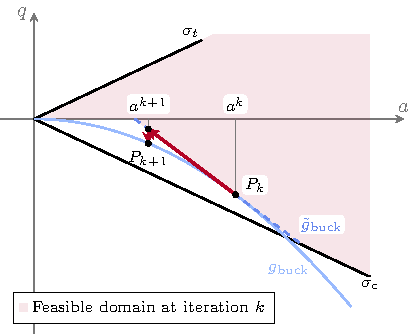
\includegraphics[width=0.7\linewidth]{figures/04_TTO_improvements/03_SLP/slp.pdf}
    \caption{Linearization of the local buckling constraints for a single bar.}
    \label{fig:04_SLP}
\end{figure}


We can now state the relaxed linearized sub-problem $\tilde{\mathbb{P}}_2$ obtained substituting \eqrefnotext{eq:04_buck} with \eqrefnotext{eq:04_buck_con_lin} in Formulation \eqrefnotext{eq:04_optim_no_constr}:
\begin{equation}
    \begin{aligned}
    \min_{\vect{a}, \vect{q}^0, \dots, \vect{q}^P}   && V &= \vect{\ell}^{T}\vect{a}\\
    \textrm{s.t.}   && \matr{B}\vect{q}^p &= \vect{f}^p && \forall p \in [0,\dots,N_p]\\
    && \vect{q}^p \geq - &\frac{s \vect{a}^k\left(2 \vect{a}^{k+1} - \vect{a}^k\right)}{\vect{\ell}^{*2}} && \forall p \in [0,\dots,N_p] \\
    && -\sigma_\text{c}\vect{a} &\leq \vect{q}^p \leq \sigma_\text{t}\vect{a} && \forall p \in [0,\dots,N_p] \\
    && a_{r}&\geq a_{r=1} && r \in \mathcal{C}_{l,r}(\vect{a}) \\
    && 0 &\leq \vect{a} \leq \frac{4 \pi \vect{\ell}^2}{\lambda_{\text{max}}}. \\
    \end{aligned}
    \tag{$\tilde{\mathbb{P}}_2$}
    \label{eq:04_optim_no_constr_lp}
\end{equation}

Since the objective function and all of its constraints are linear, we can approximate the solution of \eqrefnotext{eq:04_optim_no_constr} by iteratively solving the sub-problem \eqrefnotext{eq:04_optim_no_constr_lp}. At every iteration $k$, the vector of cross-sectional areas $\vect{a}^k$ is used to evaluate the linearization point $\vect{P}_{k}$ and calculate the set of linearized buckling constraints $\vect{\tilde{g}}_{\textrm{buck}}$ (see \figref{fig:04_SLP}). The sub-problem \eqrefnotext{eq:04_optim_no_constr_lp} is, then, solved using a \gls{lp} solver, and the updated vector of cross-sectional areas $\vect{a}^{k+1}$ is used to evaluate the set of linearized buckling constraints of the $k+1$ iteration. These steps are repeated until convergence \ie when $\norm{\Delta \vect{x}}_\infty\leq \text{tol}_{slp}$, where $\Delta \vect{x}$ represents the difference of the design variable vector $\vect{x}$ between two successive iterations. The vector $\vect{x}$ is scaled so that the difference $\Delta \vect{x}$ gives coherent results for the different physical quantities (cross-sectional areas and forces).

\subsection{Handling local minima: reinitialization strategy}
\label{sec:04_reinit}

% \begin{figure*}
%     \centering
%     \subcaptionbox{\label{fig:04_tiny-area}}{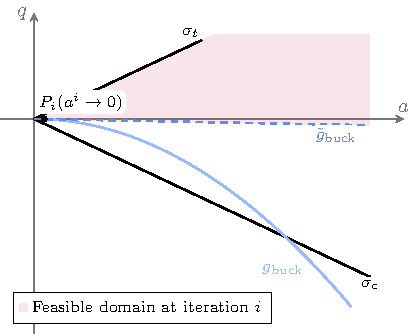
\includegraphics[width=0.45\linewidth]{figures/04_TTO_improvements/04_SLP_tiny_area_design_space/slp_tiny_design_space.pdf}}
%     \bigskip
%     \subcaptionbox{\label{fig:04_reinit_strat}}{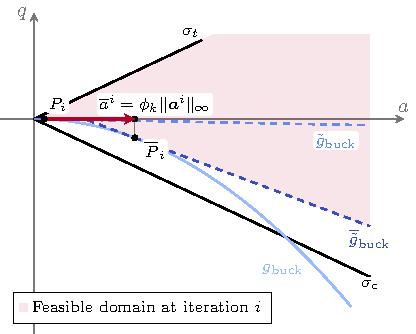
\includegraphics[width=0.45\linewidth]{figures/04_TTO_improvements/05_reinit_strategy/reinit_strat.pdf}}
%     \caption{(a) ; (b) }
% \end{figure*}
\begin{marginfigure}
    \centering
    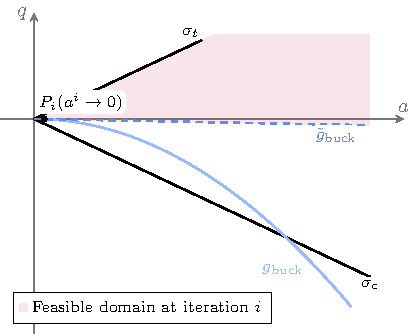
\includegraphics[width=\linewidth]{figures/04_TTO_improvements/04_SLP_tiny_area_design_space/slp_tiny_design_space.pdf}
    \caption{The linearized buckling constraints (blue dashed line) limit the design space of successive iterations when evaluated on compressive bars with very small areas. Additionally, the gradient of the linearized buckling constraint tends to 0.}
    \label{fig:04_tiny-area}
\end{marginfigure}

\begin{figure}
    \centering
    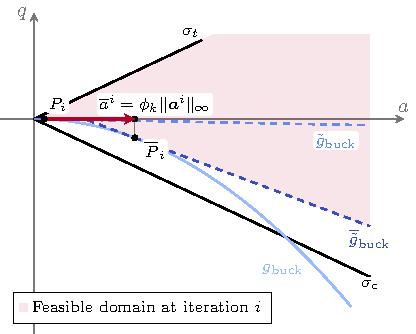
\includegraphics[width=0.7\linewidth]{figures/04_TTO_improvements/05_reinit_strategy/reinit_strat.pdf}
    \caption{The reinitialization strategy modifies the linearization point of the members with a small area to promote their reintroduction in the optimization problem.}
    \label{fig:04_reinit_strat}
\end{figure}

If at the end of iteration $k-1$ the cross-sectional area of bar $i$, $\vect{a}^k_{i}$, becomes very small, the gradient of the corresponding local buckling constraint at iteration $k$ will tend towards 0 and the feasible domain will be extremely reduced (see \figref{fig:04_tiny-area}). Any bar with near-zero sections will remain as such in future iterations since there is no incentive for the \gls{slp} optimizer to increase its value. This is one of the possible reasons why the \gls{slp} optimizer gets stuck in local minima.

Subsequently, we propose a heuristic strategy to reinitialize the small cross-sectional area values $\vect{a}^{k}$ used to evaluate the linearized local buckling constraints $\tilde{g}_{\text{buck}}$ at iteration $k$. The strategy is called multiple times during the optimization when the solver converges to a minimum, \ie when $ \norm{\Delta \vect{x}}_\infty \leq \text{tol}_{slp} $. It affects only the cross-sectional areas that are smaller than a fraction value $\tau$ of the maximum value at iteration $k$, $\norm{\vect{a^k}}_\infty$. The updated cross-sectional area $\overline{\vect{a}}^k$ used to evaluate the linearization point $\overline{\vect{P}}_{k}$ is updated as follows:
\begin{equation}
    \overline{a}^k_{i}:=
    \begin{cases}
        \phi_n \norm{\vect{a^k}}_\infty & \text{ if } a^k_{i} \leq \tau \norm{\vect{a^k}}_\infty\\
        a^i_{i} & \text { otherwise.}  
    \end{cases}
    \label{eq:04_reinit}
\end{equation}
The effects of this approach are shown in \figref{fig:04_reinit_strat}, where it is clear that updating the constraint $\tilde{g}_{\text{buck}}$ with $\overline{\tilde{g}}_{\text{buck}}$ reduces the gap between the original and the linearized design space and permits the exploration of new solutions. Additionally, the gradient of the constraint is restored to a non-zero value.

\begin{figure}
    \centering
    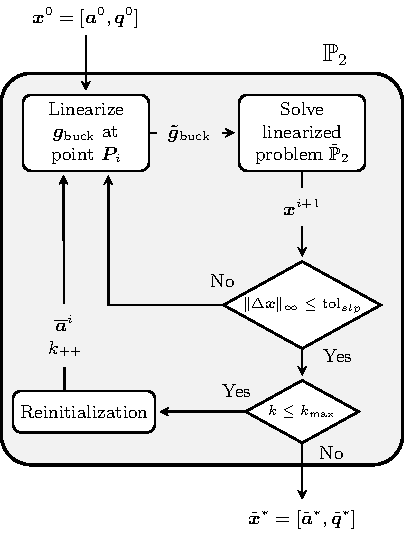
\includegraphics[width=0.7\linewidth]{figures/04_TTO_improvements/06_SLP_algo/SLP_algo.pdf}
    \caption{Flowchart of the \gls{slp} strategy with reinitialization used to solve Problem \eqrefnotext{eq:04_optim_no_constr}.}
    \label{fig:04_slp_solution}
\end{figure}

The $\phi_n$ parameter is used in \eqref{eq:04_reinit} to influence how much the reinitialization heuristic modifies the original formulation. Subsequently, to reach convergence, we propose a continuation scheme on $\phi_n$ to reduce its impact on the optimization following an exponential decay law:
\begin{equation}
    \phi_n = \phi_{n-1}^\beta \quad \forall n \in [1,\dots,n_{\text{max}}],
    \label{eq:04_phi}
\end{equation}
where $n_{\text{max}}$ represent the maximum number of reinitialization calls and the $\beta$ parameter control the steepness of the exponential progression. In that way, as the number of calls to the reinitialization strategy increases, its influence on the original formulation decreases.

The complete \gls{slp} strategy with reinitialization used to solve Problem \eqrefnotext{eq:04_optim_no_constr} is presented in \figref{fig:04_slp_solution}, where the \gls{slp} optimized design variable vector is noted as $\vect{\tilde{x}}^*=[\tilde{\vect{a}}^*, \; \tilde{\vect{q}}^*]$.

\subsection{Second step: NLP optimization}
If only one load case and no particular symmetries are imposed on the initial ground structure, the \gls{slp} solution $\vect{\tilde{x}}^*$ is not statically indeterminate \sidecite{kirsch_optimal_1989, rozvany_layout_1995}. In that case, it is trivial to evaluate the displacements using \eqrefnotext{eq:04_compatib} and the optimization is complete. However, if this is not the case, the stability of the structure is to be tested. 

The stability of the \gls{slp}-optimized structure is assessed by evaluating the \gls{dsi} of the truss using Maxwell's criterion:
\begin{equation}
    DSI= N_{\text{el}} - N_{\text{DOF}} - r
\end{equation}
with $r$ the number of fixed \gls{dofs} of the test case. If $\text{DSI}\leq0$, the number of equilibrium equations is less than or equal to the number of the internal forces and Equation \eqrefnotext{eq:04_compatib} suffices to evaluate the correct displacements of the truss. If, however, $\text{DSI}>0$, the truss is potentially statically indeterminate and additional non-linear constraints must be added to ensure the structure's kinematic compatibility. The optimization is then performed again. We call this second step the \gls{nlp} step (see \figref{fig:04_sol_alg}). 

To mitigate the risk of becoming trapped in local minima, the \gls{nlp} optimizer is employed on a reduced design space. The solution $\vect{\tilde{x}}^*$ of the \gls{slp} serves the purpose of simplifying the initial ground structure, thereby eliminating elements from the \gls{nlp} optimization that fall below the specified threshold value $a_{\text{thr}}$:
\begin{equation}
    a_i<a_{\text{thr}} \; \forall i, \text{ with }a_{\text{thr}} = \chi \; \max(\tilde{\vect{a}}^*),
    \label{eq:04_thr}
\end{equation}
with the parameter $\chi$ called the cross-sectional area threshold value.

An elastic \gls{fea} based on the direct stiffness method is performed to provide a correct estimate of forces and displacements caused by the external forces on the solution of Problem \eqrefnotext{eq:04_optim_no_constr} for the initial point of the optimization. The initial displacement vector $\vect{U}^0$ is calculated as the unique solution to:
\begin{equation}
    \vect{f}=\matr{B}^T \matr{q}=\matr{B}^{T} \matr{D} \vect{\epsilon}=\matr{B}^{T} \matr{D} \matr{B} \vect{U}^0=\matr{K} \vect{U}^0.
    \label{eq:04_truss_fem}
\end{equation} 
 where $\matr{K}$ is the stiffness matrix of the truss, defined as $\matr{K}=\matr{B}^{T} \matr{D} \matr{B}$, with $\matr{D}=\operatorname{diag}\left(E (\tilde{\vect{a}}^* + \delta \vect{e}) / \vect{\ell}\right)$, $e =[1,\dots,1]^T$, and $\delta =10^{-12}$. This last term is added as the structures coming from the \gls{slp} step could result in a mechanism with respect to load cases different from the one used for the optimization \sidecite{dorn_automatic_1964}. Then the initial member forces vector $\vect{q}^0$ is evaluated using \eqrefnotext{eq:04_compatib}. $\tilde{\vect{a}}^*, \vect{q}^0$ and $\vect{U}^0$ are used as the starting point of the full \gls{nlp} formulation where the kinematic compatibility and the exact local buckling formulation are restored. The \gls{nlp} solver finally outputs the optimized structure variables $\vect{x}^*=[\vect{a}^*,\; \vect{q}^*,\; \vect{U}^*]$.

\section{Numerical application} \label{sec:04_numerical_app}
In this section, the proposed method is benchmarked against four classical and innovative test cases. Firstly, we show how the proposed two-step solution strategy with reinitialization reduces the influence of the starting point on the optimization result compared to the direct \gls{nlp} optimization of Problem \eqrefnotext{eq:04_optim_complete}. Additionally, as the response surface of the \gls{slp} of the proposed method is more regular than the original \gls{nlp}, the two-step solution strategy generates simple structures \ie with a low number of active bars, as it is efficient at driving the cross-sectional areas to zero. To show that, we implement and optimize the ten-bar truss and the 2D cantilever beam, two of the most common benchmarks in \gls{tto} with buckling constraints. Secondly, to show the ability of the proposed method to work on structures with multiple load cases we implemented a modified ten-bar truss test case where several load cases are applied to the same ground structure. Finally, to assess the computational efficiency and to validate the proposed strategy on a large-scale structure, we optimize a three-dimensional wingbox test case based on the \acrfull{crm} with multiple discretization refinement.

The test cases are optimized using different resolution strategies. The proposed method is compared against the direct \gls{nlp} optimization of Problem \eqrefnotext{eq:04_optim_complete}, denoted in our analysis as \gls{nlp}. The proposed two-step resolution strategy is implemented with three different maximum numbers of reinitialization calls $n_{\text{max}}$: no reinitialization (2S-0R) with $n_{\text{max}}=0$, one call of reinitialization (2S-1R) with $n_{\text{max}}=1$, and finally five calls of reinitialization (2S-5R) with $n_{\text{max}}=5$. The reinitialization magnitude parameter $\vect{\phi}$ is set up using \eqref{eq:04_phi} and the parameters listed in \tabref{tab:04_param}, leading to $\phi = 0.8000$ for the 2S-1R algorithm and to $\vect{\phi} = \left[ 0.8000, 0.6400, 0.4096, 0.1677, 0.0281 \right]$ for the five reinitialization calls of 2S-5R.

The optimizations are performed using the Python package CVXPY 1.2.2 \sidecite{diamond_cvxpy_2016} with the ECOS 2.0.7 \sidecite{domahidi_ecos_2013} solver to solve the relaxed \gls{lp} Problem \eqrefnotext{eq:04_optim_no_constr_lp}. The \gls{nlp} Problem \eqrefnotext{eq:04_optim_complete} is solved using cyipopt \sidecite{Moore_Mechmotum}, a Python wrapper for IPOPT 3.14.11 \sidecite{wachter_implementation_2006}, a large-scale nonlinear optimization package using PARDISO 6.0 \sidecite{alappat_recursive_2020} as linear solver. The Jacobian and the Hessian of the Lagrangian of the \gls{nlp} step are calculated at every optimization iteration to allow faster convergence. As every state variable of the optimization is independent of the others, these responses are derived analytically and will not be detailed there. The stopping criterion used for the \gls{slp} and \gls{nlp} optimizations are $\norm{\Delta \vect{x}}_\infty \leq \text{tol}_{slp}  \text{, and } \norm{\Delta_{\text{NLP}}}_\infty \leq \text{tol}_{nlp}$, with $\text{tol}_{slp}=10^{-6}$ and $\text{tol}_{nlp}=10^{-4}$ respectively. $\Delta_{\text{NLP}}$ represents the scaled \gls{nlp} error, a more comprehensive value used by IPOPT to take into account the optimality of the solution and the constraints violation. The objective function is scaled so that the initial volume is 1000, the areas are in the interval $[0,1000]$, the initial forces in $[0,1000]$, and the displacement in $[0,1000]$ for the \gls{slp} and the \gls{nlp}. The full list of parameters used to set up the variable scaling, the \gls{slp} optimization, the reinitialization, and the \gls{nlp} optimization is listed in \tabref{tab:04_param}. Several additional parameters are used in the \gls{nlp} step for cyipopt and IPOPT:
\begin{itemize}
    \item \texttt{mu\_strategy} is set to \texttt{adaptive} 
    \item \texttt{grad\_f\_constant} is set to \texttt{yes} 
    \item \texttt{hessian\_constant} is set to \texttt{yes} 
    \item \texttt{alpha\_for\_y} is set to \texttt{min-dual-infeas}
    \item \texttt{linear\_solver} is set to \texttt{pardiso}
    \item \texttt{expect\_infeasible\_problem} is set to \texttt{yes}
    \item \texttt{bound\_push} is set to \texttt{1e-12}
    \item \texttt{constr\_viol\_tol} is set to \texttt{1e-6}
    \item \texttt{nlp\_scaling\_method} is set to \texttt{user-scaling}.
\end{itemize}

\begin{table}
    \small
\centering
\begin{tabular}{ccc}
\toprule
\textbf{Parameter} & \textbf{Value} & \textbf{Description}    \\ \midrule
$\text{tol}_{slp}$             & $10^{-6}$           & Stopping criterion \gls{slp}                       \\
$\text{tol}_{nlp}$               & $10^{-4}$           & Stopping criterion \gls{nlp}                        \\
max$_{\text{it,SLP}}$        & 400            & Maximum iterations of the \gls{slp} algorithm                       \\
max$_{\text{it,NLP}}$         & 5000           & Maximum iterations of the \gls{nlp} algorithm                        \\
$\chi$                & $10^{-6}$           & Threshold for the ground structure reduction                        \\
$\tau$                & 0.05           & Threshold for the reinitialization                        \\
$\phi_0$              & 0.8            & Initial reinitialization magnitude parameter                         \\
$\beta$             & 2              & Index of the exponential decay law \\
\bottomrule
\end{tabular}
\caption{Values and description of the parameters used for the \gls{slp} and \gls{nlp} optimizations.}
\label{tab:04_param}
\end{table}

The optimizations presented in this section are performed on a notebook equipped with an Intel\textsuperscript{\textregistered} Core™ i5-9400H Processor @ \qty{2.50}{GHz} (4 cores) and \qty{16}{GB} of RAM. Additionally, the load cases, the starting point, and the result data of all the presented test cases are available in the reference data set \sidecite{enrico_stragiotti_truss_2023}.

\subsection{L-shaped beam}

To assess the effectiveness of the proposed minimum slenderness limit, we conducted a new round of optimization on the L-shaped beam described in \secref{sec:03_applications}. In the \figref{fig:04_tto_slend}, we present the optimized structures obtained using this modified formulation and the stress limits $\sigma_\text{L}$ values of 1, 0.8, 0.3, and 0.2. The first two values have already been used and the results have been presented in \tabref{tab:03_TTO_results}. They highlighted the limits of Formulation \eqrefnotext{eq:03_optim_original} when imposing a specified slenderness limit ($\lambda<15$). The last two values are introduced here to test how the \ref{eq:04_slend_constraints} constraints affect the truss topology for extreme cases. 

A major focus is put on the shorter bar of the optimized structures to observe how the solution evolved. We observe a redistribution of the same load across multiple smaller bars. More bars became active because there is an upper limit on the cross-sectional area (and thus the force) they can withstand. The four structures present $N_\text{el,sl}=34$, 38, 56 and 79 active bars, respectively.

\begin{figure*}
    \subcaptionbox{}{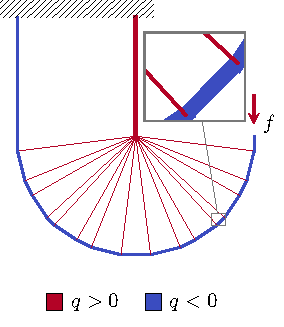
\includegraphics[width=0.23\linewidth ]{figures/04_TTO_improvements/07_slend_sol/1_opt.pdf}}
    \hfill
    \subcaptionbox{}{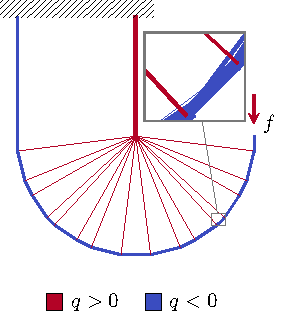
\includegraphics[width=0.23\linewidth ]{figures/04_TTO_improvements/07_slend_sol/08_opt.pdf}}
    \hfill
    \subcaptionbox{}{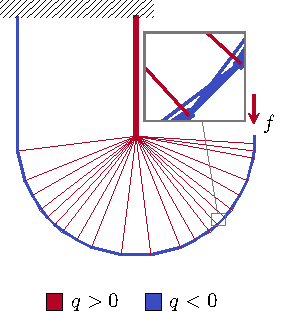
\includegraphics[width=0.23\linewidth ]{figures/04_TTO_improvements/07_slend_sol/03_opt.pdf}}
    \hfill
    \subcaptionbox{}{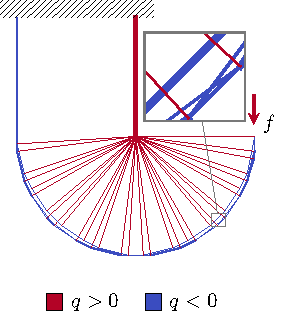
\includegraphics[width=0.23\linewidth ]{figures/04_TTO_improvements/07_slend_sol/02_opt.pdf}}
    \caption{Topology of the optimized truss structures for different material admissibles $\sigma_\text{L}=1.0,0.8,0.3\text{ and }0.2$ with a minimum slenderness limit $\lambda<15$.}
    \label{fig:04_tto_slend}
\end{figure*}

In \tabref{tab:04_TTO_l_slend} we compared the new designs limited in minimum slenderness (noted in the table with the 'sl' subscript) to the ones presented in \secref{sec:03_applications} and found that the new designs meet the bar model's slenderness requirements correctly. The number of active bars increases along with the calculation time, but the volume remains nearly the same, indicating there are many solutions with similar volumes. Adding this upper bound constraint, we have extended the domain of application of the \gls{tto}. However, we must be careful because very high volumes of fraction solutions can lead to too many bar intersections, resulting in structures with no physical meaning.

\begin{table*}
    \small
    \centering
    \sisetup{table-auto-round}
    \begin{tabular}{S[table-format = 2.1]
                    S[table-format = 2.2]
                    S[table-format = 2.1] 
                    S[table-format = 2.2]
                    S[table-format = 2.1]                    
                    S[table-format = 1.4]
                    S[table-format = 1.2]
                    S[table-format = 1.2]}
                    \toprule
    $\bm \sigma_L$&$\bm V_\text{f}$  & {\textbf{Min} $\bm \lambda$} & $\bm V_\text{f,sl}$  & {\textbf{Min} $\bm \lambda_\text{sl}$}&$\bm V_\text{f,sl}/\bm V_\text{f}$&$\bm N_\text{el,sl}/\bm N_\text{el}$&$\bm t_\text{sl}/\bm t$\\ \midrule
    1           & 6.208431\ppercent  & 15.795                    & 6.208431\ppercent& 15.795  &1&1       &1.02            \\
    0.90        & 6.898257\ppercent  & 14.984                    & 6.898257\ppercent& 14.984  &1&1       &1.03            \\
    0.80        & 7.760539\ppercent  & \color{accent_r_1}14.127  & 7.761069\ppercent& 15.0    &1,0000682&1,1176       & 2.27    \\
    0.70        & 8.869187\ppercent  & \color{accent_r_1}13.215  & 8.870386\ppercent& 15.0    &1,0001351&1,1176       & 2.21    \\
    0.60        & 10.347385\ppercent & \color{accent_r_1}12.235  &10.349476\ppercent& 15.0    &1,0002020&1,1176      & 1.12    \\
    0.50        & 12.416862\ppercent & \color{accent_r_1}11.169  &12.420203\ppercent& 15.0    &1,0002690&1,1176      & 1.07    \\
    0.4         & {--}      & {--}                               &15.526292\ppercent& 15.0    &{--}&{--} &{--}                 \\
    0.3         & {--}      & {--}                               &20.705531\ppercent& 15.0    &{--}&{--} &{--}        \\ 
    0.2         & {--}      & {--}                               &31.061628\ppercent& 15.0    &{--}&{--} &{--}                \\ \bottomrule
    \end{tabular}
    \caption{Numerical comparison of the effect of the minimum slenderness constraint on the optimization of the 2D L-shaped beam.}
    \label{tab:04_TTO_l_slend}
\end{table*}

\subsection{Ten-bar truss}
\label{sec:04_10bar}
 \begin{figure}
    \centering
    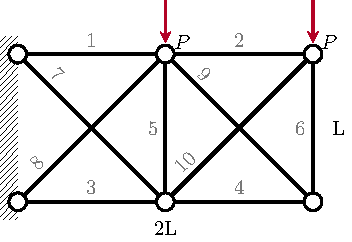
\includegraphics{figures/04_TTO_improvements/08_10_bar/10_bar_BC.pdf}
    \caption{The ten-bar truss ground structure and load case.}
    \label{fig:04_10-bar-bcs}
\end{figure}
The ten-bar truss is a test case subjected to maximum stress and local buckling constraints proposed by \cite{guo_new_2001} and is shown in \figref{fig:04_10-bar-bcs}. It is a small test case with 32 design variables (10 cross-sectional area, 10 internal force, and 12 displacement variables) and 42 constraints (12 force equilibrium, 20 maximum stress, 10 local buckling, and 10 kinematic compatibility constraints) when solved using Formulation \eqrefnotext{eq:04_optim_complete}. The geometry and material data are given in \tabref{tab:04_10-bar_mat}. For simplicity, all numeric values are assumed normalized and dimensionless. We compare the results obtained by our method with those obtained by direct \gls{nlp} resolution and with the results published by \cite{guo_new_2001} and \cite{stolpe_note_2003}. 

\begin{margintable}
    \small
    \centering
    \begin{tabular}{cc}
    \toprule
    \textbf{Parameter}        & \textbf{Value} \\ \midrule
    $L$ & 360 \\
    $E$              & $1.0 \times 10^{4}$     \\
    $s$ & $\pi E/4$ \\
    $\sigma_\text{c}, \sigma_\text{t}$ & $\pm 20$ \\
    $P$              & 100   \\
    \bottomrule
    \end{tabular}
    \caption{Material data used for the ten-bar truss optimization.}
    \label{tab:04_10-bar_mat}
\end{margintable}

The robustness of the optimization algorithms to local minima is evaluated by running 50 optimizations from different initialization points $\vect{a}^0$ randomly chosen in the interval $[0,\;100]$. The first initialization point, denoted $\vect{a}^0_s$, is specifically chosen to match the one used by \cite{stolpe_note_2003} ($a_{s,2}^0=a_{s,8}^0=a_{s,10}^0=0$ and $a_{s,i}^0=50$ elsewhere). This is the starting point from which the authors conclude that the problem is initialization-dependent. 

\begin{figure}
    \centering
    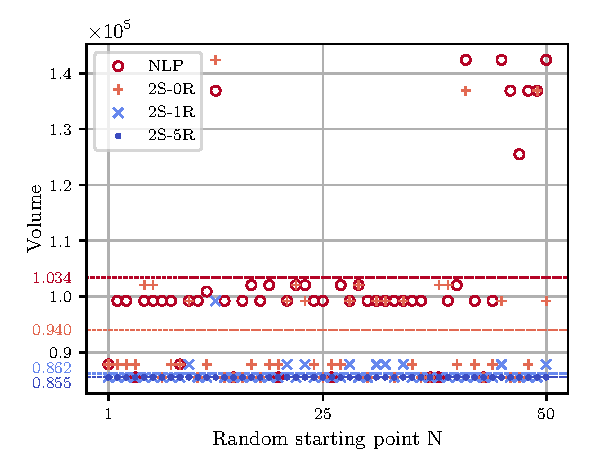
\includegraphics{figures/04_TTO_improvements/09_Convergence_10bars/10bar-conv.pdf}
    \caption{Scatter plot of the four benchmarked optimization algorithms on the ten-bar truss. The 2S-5R shows a \qty{100}{\%} convergence rate to the lightest structure found. The dashed lines represent the mean of the distributions.}
    \label{fig:04_10_bar_convergence}
\end{figure}

\begin{table}
    \small
\centering
\begin{tabular}{ccS
S[table-format = 2.0]
S[table-format = 1.2]}
\toprule
\textbf{Algorithm} &
  \multicolumn{1}{c}{$\bm{\overline{V}} \pm \textbf{SD}$} &
  \multicolumn{1}{c}{\textbf{Conv.}} &
  \multicolumn{1}{c}{$\textbf{It.}$} &
  \multicolumn{1}{c}{$\textbf{t [\unit{\second}]}$}\\ \midrule
NLP & $(1.03\pm0.15) \times 10^5$&\qty{14}{\percent} &22&0.25 \\
2S-0R & $(9.40\pm1.22) \times 10^4$&\qty{20}{\percent} &4&0.06 \\
2S-1R & $(8.62\pm0.21) \times 10^4$&\qty{80}{\percent} &17&0.24 \\
2S-5R & $(8.55\pm0.00) \times 10^4$&\qty{100}{\percent} &73&1.18  \\
\midrule
\cite{guo_new_2001} &$8.78\times 10^4$&{-}&{-}&{-} \\
\cite{stolpe_note_2003} &$8.55\times 10^4$&{-}&{-}&{-} \\
\bottomrule
\end{tabular}
\caption{Numerical comparison of the four optimization algorithms on the ten-bar truss for 50 different initial points. The 2S-5R algorithm shows a \qty{100}{\%} convergence rate to the lightest structure found. The iteration count and time are from the first initialization point $\vect{a}^0_s$.}
\label{tab:04_10_bar_solution}
\end{table}

In \figref{fig:04_10_bar_convergence} we show the scatter plot of the optimization of the ten-bar truss for the four considered resolution algorithms, where for every initialization point (X-axis) we show the final volume of the structure. The \gls{nlp} algorithm converges to different solutions with varying volume values, confirming an abundance of local minima even for such a small test case with 10 bars. The optimized results are dispersed, and the best design found ($V=85534$) is only attained 7 times over the 50 optimization runs (\qty{14}{\%}). To properly compare the different algorithms, we use two different figures of merit: the mean $\overline{V}$ and the standard deviation SD of the distribution of the volume of the optimized designs and the ratio of solutions converged to the best result to the total number of initialization points. The numerical results are listed in \tabref{tab:04_10_bar_solution}. The proposed two-step optimization strategy (2S-0R) already reduces $\overline{V}$ by approximately \qty{9}{\%} compared to \gls{nlp}, but it is only when we introduce the reinitialization strategy that major improvements are observed, especially when multiple calls of the heuristic are done. The five-calls reinitialization optimization strategy (2S-5R) is not influenced by the initialization point ($\text{SD}=0$), with all solutions successfully converging to the lightest structure.

\begin{figure*}
    \centering
    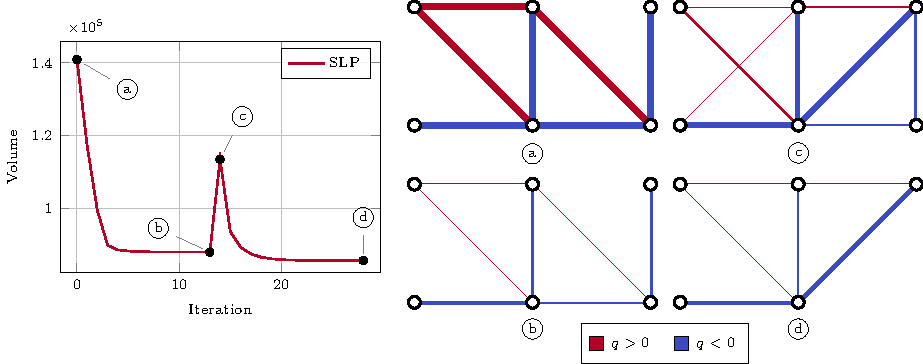
\includegraphics{figures/04_TTO_improvements/10_10_bar_history/10_bar_hist.pdf}
    \caption{Volume convergence history for the proposed two-step resolution strategy with one step of reinitialization (2S-1R) for the initialization point $\vect{a}^0_s$. The reinitialization strategy permits to jump from the local minimum (b), with $V=87857$, to the lighter structure (d), with $V=85534$. Only the \gls{slp} step is plotted because the solution is statically determinate and kinematic compatibility constraints are already satisfied. In red the members loaded in tension, in blue the members loaded in compression.}
    \label{fig:04_10_bar_hist}
\end{figure*}

Let us consider only the first initialization point $\vect{a}^0_s$. In \figref{fig:04_10_bar_hist} we show the convergence history and the design of the structure throughout the iterations for that specific case. We notice how the initialization point $\vect{a}^0_s$ (represented in \figref{fig:04_10_bar_hist}a) corresponds to the topology of the local minimum found by \cite{guo_new_2001}. As extensively shown in \secref{sec:04_reinit}, if the cross-sectional area of one member is almost or exactly zero the gradient of the local buckling constraint tends to zero and the bar is not considered in the optimization anymore. For that reason, the optimizer is not able to restore the bars initialized at 0 and promptly converges to a solution that presents the very same topology (see \figref{fig:04_10_bar_hist}b, $V=87857$). This structure would be the optimization result if no additional steps are done. With a single call of the reinitialization heuristic, the topology is modified as shown in \figref{fig:04_10_bar_hist}c, in which bars 2 and 10 are reintroduced in the set of active members. From this iteration, the optimizer finally converges to the lighter structure shown in \figref{fig:04_10_bar_hist}d with $V=85534$, showing the interest of the reinitialization strategy. We notice how only the \gls{slp} step of the proposed two-step strategy is shown here as the optimized structure is statically determinate (\gls{dsi}=0 and stiffness matrix $\matr{K}$ non-singular) and the kinematic compatibility is already satisfied by the optimized design.

It should be mentioned that the proposed heuristic comes with an increase in computational cost. While for the first initialization point, the 2S-0R algorithm converges in only 4 iterations, the single-step 2S-1R and the five-step 2S-5R algorithms converge after 17 and 73 iterations, respectively. The optimization time is slightly more than one second (see the last column of \tabref{tab:04_10_bar_solution}). However, this increase in calculation time is justified by the fact that a single initialization point should suffice to reach an acceptable solution, instead of using a multistart approach.

It is advisable to select the highest number of reinitialization calls (parameter $n_{\text{max}}$ of \eqref{eq:04_phi}) that is compatible with the user's computational budget. Our research findings suggest that once the parameter $\phi_k$ (which determines the strength of the heuristic perturbation) drops below 0.01, the reinitialization has no more influence on the result of the linearized problem. Therefore, with the proposed parameterization of the continuation scheme, pursuing more than five reinitialization calls does not yield additional benefits in the studied test cases.

\subsection{2D cantilever beam}
\label{sec:04_2dcant}
\begin{margintable}
    \small
    \centering
    \begin{tabular}{cc}
    \toprule
    \textbf{Parameter}        & \textbf{Value} \\ \midrule
    $L$ & 1 \\
    $E$              & $(12\sqrt{2})/(\pi^2)$     \\
    $s$ & $\pi^2 E / 12$ \\
    $\sigma_\text{c}, \sigma_\text{t}$ & $\pm 1$ \\
    $P$              & 1   \\
    \bottomrule
    \end{tabular}
    \caption{Material data used for the 2D cantilever beam optimization.}
    \label{tab:04_2D_cand_mat}
\end{margintable}

The second example we consider is a 2D cantilever beam charged on one extremity as shown in \figref{fig:04_2d_cant}. This test case was proposed by Achtziger \sidecite{achtziger_local_1999b} with the geometry and dimensionless material data given in \tabref{tab:04_2D_cand_mat}. The number of the candidate bars of the initial ground structure is $N_{\text{el}}=90$. The complexity of this problem resides in the fact that the geometry and material data are chosen in such a way that the solution with or without local buckling constraints coincides if topological buckling is not considered. The optimized structure shows in this case a volume of $V=70.00$. However, as this structure presents multiple bars in compressive chains, we need to merge them into single bars, recalculate their length, and evaluate their sections to comply with local buckling constraints. By doing so, we would obtain $V=99.99$, an increase of more than \qty{40}{\%} with respect to the optimized structure just found. This load case is built to show the importance of topological buckling and suggests that a lighter solution is to be found between these two bounds.
\begin{figure}
    \centering
    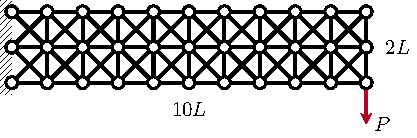
\includegraphics{figures/04_TTO_improvements/11_Ach_cant/Ach_BC.pdf}
    \caption{The 2D cantilever beam load case with a first-order connectivity ground structure. The total number of candidate members is $N_{\text{el}}=90$.}
    \label{fig:04_2d_cant}
\end{figure}

\begin{table}
    \small
\centering
\begin{tabular}{cSS[table-format = 2.2(1), separate-uncertainty]S[table-format = 2.0]S[table-format = 2.2(1), separate-uncertainty]}
\toprule
\textbf{Algorithm} &
  \multicolumn{1}{c}{$\bm{V_{\text{min}}}$} &
  \multicolumn{1}{c}{$\bm{\overline{V}}\pm \textbf{SD}$} &
  \multicolumn{1}{c}{$\bm{N_{\text{min}}}$} &
  \multicolumn{1}{c}{$\bm{\overline{N}_{\text{el}}}\pm \textbf{SD}$} \\ \midrule
NLP & 80.67 & 81.34\pm2.98  & 58 & 66.57\pm1.13 \\
2S-0R & 79.88 & 92.80 \pm7.45 & 10 & 25.61\pm7.94 \\
2S-1R & 77.78 & 88.42\pm6.29  & 10 & 27.86\pm6.56 \\
2S-5R & 77.78 & 86.72\pm6.05  & 10 & 28.60\pm6.44  \\
\midrule
\cite{achtziger_local_1999b} &85.58&{-}&18&{-}  \\\bottomrule
\end{tabular}
\caption{Numerical comparison of the 2D cantilever beam of the four algorithms for 100 random initial points. The 2S-5R algorithm shows a good balance between the volume, complexity, and dispersion of the solutions.}
\label{tab:04_2d_cant_solution}
\end{table}

The 2D cantilever is optimized starting from 100 random points $\vect{a}^0 \in [0,\;100]$ and the same four algorithms presented in the previous section. At the end of the optimization, the resulting structures are checked for compressive chains and, if present, they are merged into single bars. The final volume does not change as the effective buckling length $\ell^*$ is iteratively updated using \eqref{eq:04_chain_len} during the optimization. The numerical results are presented in \tabref{tab:04_2d_cant_solution}.

\begin{figure*}
    \centering
    \hspace*{\fill}
    \subcaptionbox{\label{fig:04_2d_cant_nlp}}{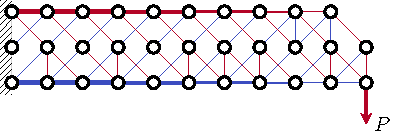
\includegraphics{figures/04_TTO_improvements/12a_Ach_cant_nlp/Ach_BC_nlp.pdf}}
    \hfill
    \subcaptionbox{\label{fig:04_2d_cant_opt}}{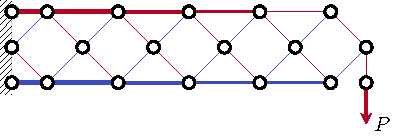
\includegraphics{figures/04_TTO_improvements/12b_Ach_cant_opt/Ach_BC_opt.pdf}}
    \hspace*{\fill}
    \caption{(a) \gls{nlp} optimized design of the 2D cantilever beam with a volume of $V=80.67$ and high number of active and crossing bars $N_{\text{el}}=66$; (b) 2S-5R solution $V=77.78$ with $N_{\text{el}}=31$. In red the members loaded in tension, in blue the members loaded in compression.}
    \label{fig:04_2d_cant_sol}
\end{figure*}

\begin{margintable}
    \resizebox{\linewidth}{!}{
    \centering
    \addtolength{\tabcolsep}{-0.5em}
    \begin{tabular}{ccSSSS}
    \toprule
    \multicolumn{1}{c}{\textbf{($x_a$ $y_a$)}} &
      \multicolumn{1}{c}{\textbf{($x_b$ $y_b$)}} &
      \multicolumn{1}{c}{\textbf{$\ell$}} &
      \multicolumn{1}{c}{\textbf{q}} &
      \multicolumn{1}{c}{\textbf{a}} &
      \multicolumn{1}{c}{\textbf{V}} \\ \midrule
    (0 0)  & (1 0)  & 1.00 & -5.00 & 5.00 & 5.00 \\
    (1 0)  & (0 1)  & 1.41 & 0.71  & 0.71 & 1.00 \\
    (1 0)  & (2 1)  & 1.41 & -0.71 & 1.02 & 1.45 \\
    (3 0)  & (2 1)  & 1.41 & 0.71  & 0.71 & 1.00 \\
    (3 0)  & (4 1)  & 1.41 & -0.71 & 1.02 & 1.45 \\
    (5 0)  & (4 1)  & 1.41 & 0.71  & 0.71 & 1.00 \\
    (5 0)  & (6 1)  & 1.41 & -0.71 & 1.02 & 1.45 \\
    (7 0)  & (6 1)  & 1.41 & 0.71  & 0.71 & 1.00 \\
    (7 0)  & (8 1)  & 1.41 & -0.71 & 1.02 & 1.45 \\
    (9 0)  & (8 1)  & 1.41 & 0.71  & 0.71 & 1.00 \\
    (9 0)  & (10 1) & 1.41 & -0.71 & 1.02 & 1.45 \\
    (10 0) & (10 1) & 1.00 & 1.00  & 1.00 & 1.00 \\
    (0 1)  & (1 2)  & 1.41 & -0.71 & 1.02 & 1.45 \\
    (2 1)  & (1 2)  & 1.41 & 0.71  & 0.71 & 1.00 \\
    (2 1)  & (3 2)  & 1.41 & -0.71 & 1.02 & 1.45 \\
    (4 1)  & (3 2)  & 1.41 & 0.71  & 0.71 & 1.00 \\
    (4 1)  & (5 2)  & 1.41 & -0.71 & 1.02 & 1.45 \\
    (6 1)  & (5 2)  & 1.41 & 0.71  & 0.71 & 1.00 \\
    (6 1)  & (7 2)  & 1.41 & -0.71 & 1.02 & 1.45 \\
    (8 1)  & (7 2)  & 1.41 & 0.71  & 0.71 & 1.00 \\
    (8 1)  & (9 2)  & 1.41 & -0.71 & 1.02 & 1.45 \\
    (10 1) & (9 2)  & 1.41 & 0.71  & 0.71 & 1.00 \\
    (0 2)  & (1 2)  & 1.00 & 5.00  & 5.00 & 5.00 \\
    (1 0)  & (3 0)  & 2.00 & -4.00 & 4.00 & 8.00 \\
    (3 0)  & (5 0)  & 2.00 & -3.00 & 3.00 & 6.00 \\
    (5 0)  & (7 0)  & 2.00 & -2.00 & 2.43 & 4.87 \\
    (7 0)  & (9 0)  & 2.00 & -1.00 & 1.72 & 3.44 \\
    (1 2)  & (3 2)  & 2.00 & 4.00  & 4.00 & 8.00 \\
    (3 2)  & (5 2)  & 2.00 & 3.00  & 3.00 & 6.00 \\
    (5 2)  & (7 2)  & 2.00 & 2.00  & 2.00 & 4.00 \\
    (7 2)  & (9 2)  & 2.00 & 1.00  & 1.00 & 2.00 \\ \midrule
    \multicolumn{1}{c}{} &
      \multicolumn{1}{c}{} &
      \multicolumn{1}{c}{} &
      \multicolumn{1}{c}{} &
      \multicolumn{1}{c}{$\bm{V_{\text{tot}}}$} &
      77.78\textsuperscript{\emph{a}} \\ \bottomrule
    \end{tabular}}
    \\
    \scriptsize{\textsuperscript{\emph{a}}The total volume value is lower than the sum of the member volumes due to the 2 decimal places round-off.}
    \caption{Optimal values of the member forces, areas, and volumes of the 2D cantilever beam.}
    \label{tab:04_2d_cant_opt}
\end{margintable}

\begin{figure*}
    \centering
    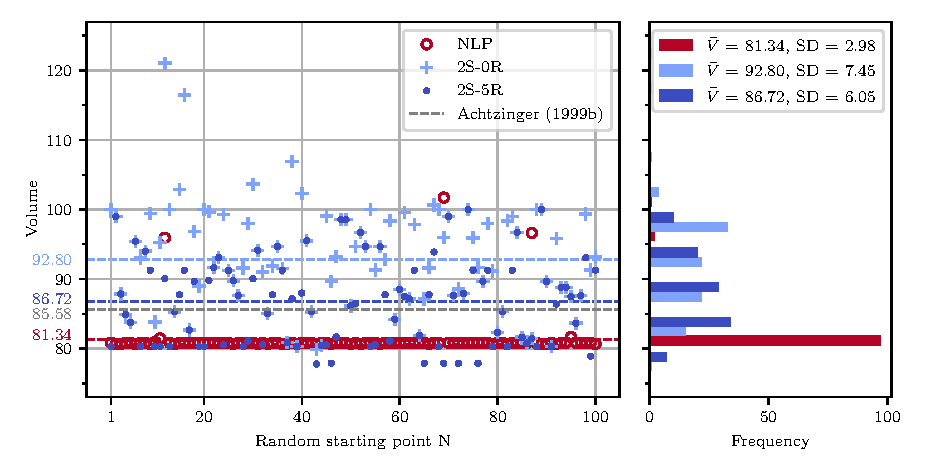
\includegraphics{figures/04_TTO_improvements/13_convergence_Achtz/cant_ach-conv.pdf}
    \caption{Left: scatter plot of three of the four benchmarked optimization algorithms on the 2D cantilever beam compared to the solution by Achtziger \cite{achtziger_local_1999b}. The dashed lines represent the mean of distributions. Right: histogram of the distribution of the results of the optimization algorithms.}
    \label{fig:04_2d_cant_convergence}
\end{figure*}

The \gls{nlp} algorithm shows a good consistency with a mean volume $\overline{V}=81.34$ and a low dispersion of the results ($\text{SD}=2.98$), repeatedly converging to a specific solution with $V=80.85$. However, despite the apparent good numerical performance, the solutions always present a high number of active bars, with an average $\overline{N}_{\text{el}}$ of over 66 bars. As discussed in \secref{sec:04_method}, the \gls{nlp} algorithm encounters difficulties in driving the cross-sectional areas to 0. \figref{fig:04_2d_cant_nlp} shows the lightest design found using \gls{nlp}, with $V = 80.67$ and $N_{\text{el}}=66$.

The proposed two-step formulation without reinitialization 2S-0R drastically reduces the complexity of the structure, with an average number of active bars $\overline{N}_{\text{el}}$ of around 27, and an absolute minimum of $N_{\text{min}}=10$. However, this simplification of the design comes at the expense of an increased average volume and dispersion ($\overline{V}=92.80$ and $\text{SD}=7.45$). This detrimental effect is efficiently counterbalanced with the proposed reinitialization strategy, which reduces the average volume to $\overline{V}=86.72$ and $\text{SD}=6.05$ for 2S-5R. To sum up, the \gls{nlp} remains stuck in a low-volume local optimum whose volume varies little and that shows a very high number of active bars. With the two-stage strategy, the number of bars of the optimized structures is \qty{58}{\%} lower, resulting in a lighter design in \qty{30}{\%} of cases, and with the best design found that is \qty{3.5}{\%} lighter.

\figref{fig:04_2d_cant_convergence} shows how the results of the proposed algorithm are more scattered and do not converge to a single minimum as precedently seen on the ten-bar truss example of \secref{sec:04_10bar}. A possible explanation for this difference in performance might be the discrete nature of the optimization when topological buckling constraints are taken into account. In some rare cases, we observed that calling the reinitialization makes the optimization converge to a more voluminous design compared to the one we had just before. In these cases, the results presented are the best ones encountered over the optimization steps and not the final ones.

The lightest solution found by 2S-5R with a volume of $V=77.78$ and with $N_{\text{el}}=31$ is presented in \figref{fig:04_2d_cant_opt}. Some of the active members of the optimized design are not present in the original ground structure but are the result of the bar merging process. The optimized design shows a \qty{9}{\%} lower volume with respect to the solution found by Achtziger \sidecite{achtziger_local_1999b} with $V=85.57$\sidenote{Even if Achtziger \cite{achtziger_local_1999b} reports an optimized volume of $V=79.57$, we use here the value corrected by Tyas \cite{tyas_practical_2006} of $V=85.57$.}. The detailed value of the design variables of the solution can be found in \tabref{tab:04_2d_cant_opt} and in the referenced data set \sidecite{enrico_stragiotti_truss_2023}. Approximately \qty{45}{\%} of the solutions of the 2S-5R algorithm are less voluminous than the one found by Achtziger.

The authors are aware of the less voluminous solution ($V=73.44$) found by \cite{tyas_practical_2006}. The main reason for the difference is that Tyas's method allows the inclusion of bracing-only members that are not required for primary load-carrying purposes to reduce the effective buckling lengths $\ell$ of internal members. The incorporation of these members is regulated by introducing perturbative forces applied to the structure as additional load cases at unstable nodes. In the specific example of Tyas' structure, the resulting structure is statically admissible, and this ensures that kinematic compatibility is satisfied. However, as demonstrated later in this Chapter, this may not always be the case. Tyas' formulation, in this context, serves only as a lower-bound formulation for minimizing the structure's volume.

\subsection{Simply supported 3D beam} \label{sec:04_simply_supp}
In this subsection, we focus on optimizing a simply supported three-dimensional beam. The supports are positioned at all four lower extremities of the design volume, the structure is subjected to five equispaced nodal loads, with each load magnitude set to $P=\qty{100}{N}$, applied on the XZ symmetry plane of the structure, as depicted in \figref{fig:04_simply3D_BC}. The volume of the design space is \qty{150}{mm} x \qty{50}{mm} x \qty{75}{mm}. These specific dimensions have been selected to accommodate the printing volume of the Creality Halot One, which is an \gls{sla} 3D printer with maximal printing dimensions of \qty{127}{mm} x \qty{80}{mm} x \qty{160}{mm}.
\begin{figure}
    \centering
    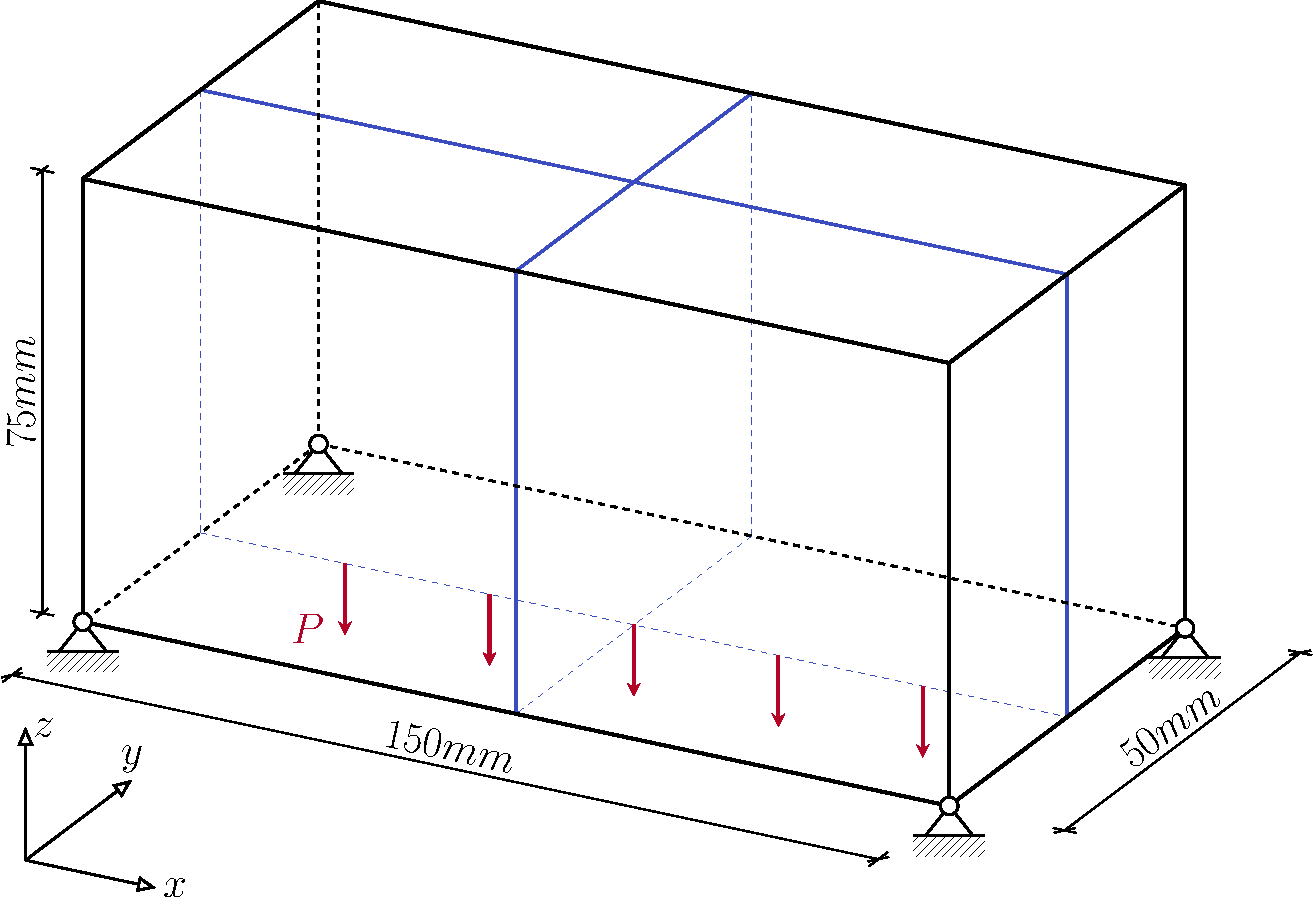
\includegraphics[width=0.8\linewidth]{figures/04_TTO_improvements/14_supported_3D_BCs/supported_3D.pdf}
    \caption{The simply supported 3D beam example with the load case and boundary conditions. In blue we plot the symmetry planes.}
    \label{fig:04_simply3D_BC}
\end{figure}
The material properties used for the optimization are given in \tabref{tab:04_3D_supp_mat} and mimic a tough \gls{sla} resin \sidenote{The material data has been sourced from \href{https://www.3ds.com/make/solutions/blog/sla-3d-printing-materials-compared}{3ds.com/make/solutions/blog/sla-3d-printing-materials-compared} and \href{https://hubs.com/knowledge-base/sla-3d-printing-materials-compared}{hubs.com/knowledge-base/sla-3d-printing-materials-compared}.}. The test case exhibits symmetry concerning the XZ and YZ planes (see blue lines of \figref{fig:04_simply3D_BC}), enabling us to mesh and optimize just one-quarter of the structure. This specific portion is meshed using a fully connected ground structure with dimensions of 4x2x4 nodes, resulting in a total of 496 elements (or 1984 for the entire structure). For this case, we employ the 2S-5R solving algorithm.

\begin{marginfigure}
    \centering
    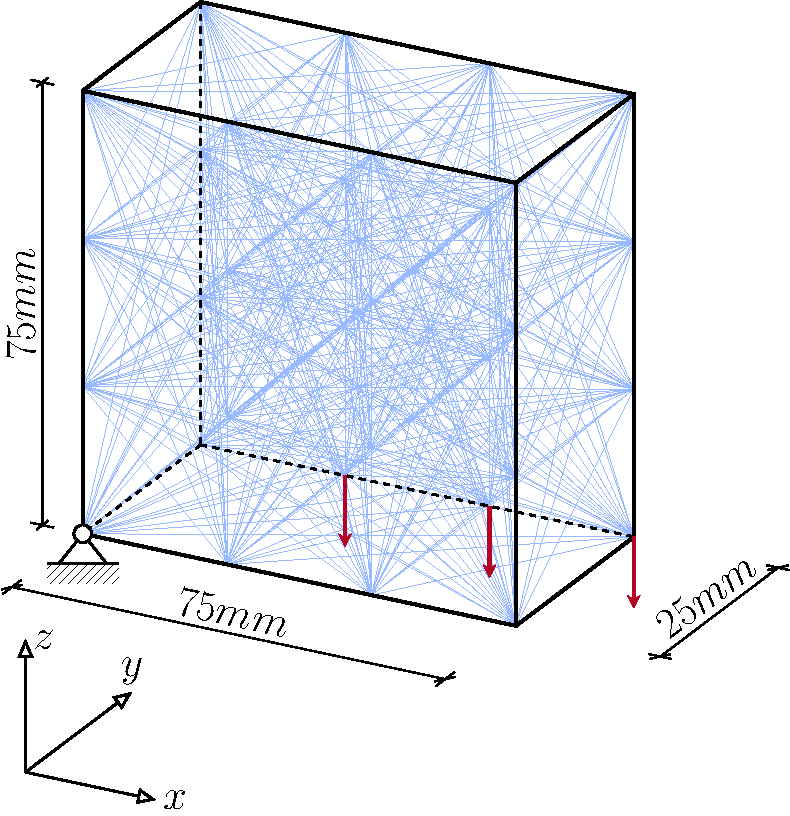
\includegraphics[width=\linewidth]{figures/04_TTO_improvements/15_supported_3D_BCs_symm/supported_3D_symm.pdf}
    \caption{Ground structure composed of $N_\text{el}=496$ elements of the symmetric portion used to optimize the simply supported 3D beam.}
    \label{fig:04_simply3D_BC_GS}
\end{marginfigure}

\begin{margintable}
    \small
    \centering
    \begin{tabular}{cc}
    \toprule
    \textbf{Parameter}        & \textbf{Value} \\ \midrule
    $E$              & \qty{2.7}{GPa}     \\
    $\nu$            & 0.3   \\
    $\sigma_\text{c}, \sigma_\text{t}$ & $\pm $\qty{55}{MPa} \\
    $\rho$              & \qty{1.14}{\gram\per\cubic\centi\metre}   \\
    $P$              & \qty{100}{N}   \\
    \bottomrule
    \end{tabular}
    \caption{Material data used for the simply supported 3D beam optimization.}
    \label{tab:04_3D_supp_mat}
\end{margintable}

\tabref{tab:04_3D_supp_res} and \figref{fig:04_3D_supp_topo} show the numerical results and topology of the optimized structure, respectively. The entire structure features 20 active bars, approximately 1 percent of the original ground structure. In \figref{fig:04_3D_supp_mech}, we visualize the stress and buckling constraints applied to the optimized structure. Every compression-loaded bar of the optimized structure activates the buckling constraint, underscoring the critical importance of accounting for this mode of structural failure in a truss. The final structure has a weight of \qty{11.294}{\gram} and achieves a volume fraction of \qty{1.761}{\%}. The optimization process is completed within 4 seconds, with only the \gls{slp} solved, as the resultant structure is statically determinate and kinematic constraints are inherently satisfied.

\begin{table}
    \small
    \centering
    \begin{tabular}{cc}
    \toprule
    \textbf{Quantity} & \textbf{Value}  \\ \midrule
    N$_{\text{el}}$  & 1984                   \\
    N$_{\text{opt}}$ & 20                     \\
    V &  \qty{9.907}{\centi\meter^3}                    \\
    V$_\%$   &   \qty{1.761}{\%}    \\
    Mass  &   \qty{11.294}{\gram}    \\
    a$_{\text{max}}$& \qty{37.61}{\milli\meter^2}       \\
    C         &  \qty{3.71}{\joule}             \\
    t  & \hms{0;0;4}          \\ \bottomrule            
    \end{tabular}
    \caption{Numerical results of the optimization of the simply supported 3D beam.}
    \label{tab:04_3D_supp_res}
\end{table}

\begin{figure*}
    \centering
    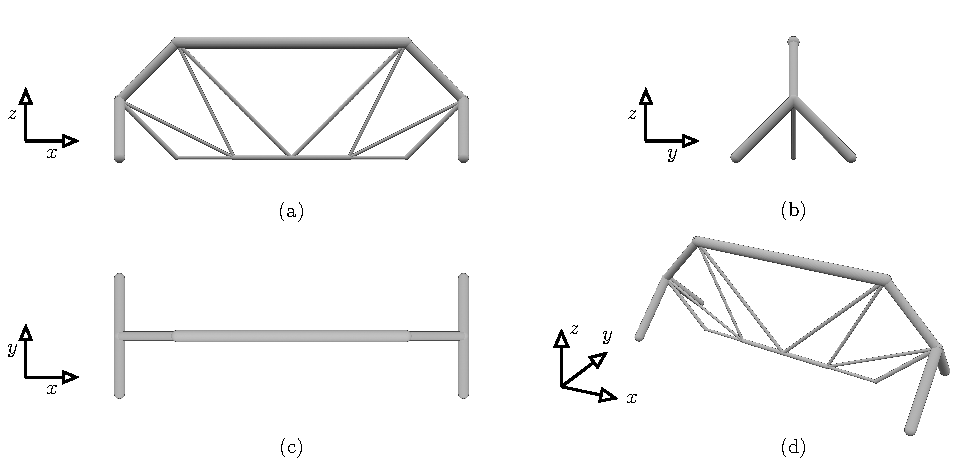
\includegraphics{figures/04_TTO_improvements/16_supported_3D_sol/support_sol.pdf}
    \caption{Orthographic views of the topology of the optimized simply supported 3D beam. (a) XZ plane (b) YZ plane (c) XY plane (d) auxiliary perspective view.}
    \label{fig:04_3D_supp_topo}
\end{figure*}

\begin{figure*}
    \centering
    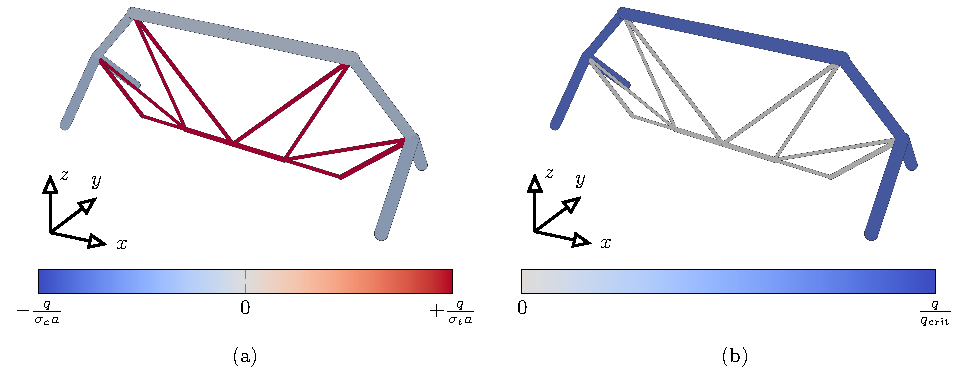
\includegraphics[width=0.90\linewidth]{figures/04_TTO_improvements/17_supported_3D_mech/support_mech.pdf}
    \caption{Maximum stress constraint value (a) and buckling constraint value (b) plotted on the optimized topology of the simply supported 3D beam.}
    \label{fig:04_3D_supp_mech}
\end{figure*}

\subsection{Ten-bar truss with multiple load cases}
\label{sec:04_10multi}

We introduce here a more complex example to validate the proposed algorithm on a multiple load cases structure with maximum stress and topological buckling constraints. The test case is obtained by slightly modifying the ten-bar truss presented in \secref{sec:04_10bar}. The ground structure and the material data are the same, and two load cases $P_1$ and $P_2$ are applied at the structure's free extremity in a symmetric way with respect to the horizontal axis. A graphical presentation of the load case is shown in \figref{fig:04_10-bar-bcs-multi}. The loads' magnitude is set to $P_1=P_2=1$.

First, we optimize the structure using the same four algorithms and the starting point presented in Section \ref{sec:04_10bar}. Differently from the structures optimized earlier in Sections \ref{sec:04_10bar} and \ref{sec:04_2dcant}, the solutions of the \gls{slp} step are statically indeterminate, as they show a $\text{DSI}>0$ and a non-singular $\matr{K}$ stiffness matrix. For that reason, the structures undergo a second optimization in which the kinematic compatibility and the exact buckling constraints are restored (NLP step, see Formulation \eqrefnotext{eq:04_optim_complete}). The numerical findings of the four algorithms are presented in Table \ref{tab:04_10_bar_multi_solution}.

\begin{table}
    \small
\centering
\begin{tabular}{cc}
\toprule
\textbf{Algorithm} &
  \multicolumn{1}{c}{$\bm{\overline{V}} \pm \textbf{SD}$}\\ \midrule
NLP & $1.45\times 10^5\pm1.44\times 10^4 $ \\
2S-0R & $1.33\times 10^5\pm9.56\times 10^3 $ \\
2S-1R & $1.35\times 10^5\pm2.73\times 10^3 $ \\
2S-5R & $1.35\times 10^5\pm2.73\times 10^3 $ \\
\bottomrule
\end{tabular}
\caption{Numerical comparison of the four optimization algorithms on the ten-bar truss for 50 different initial points.}
\label{tab:04_10_bar_multi_solution}
\end{table}

\begin{figure}
    \centering
    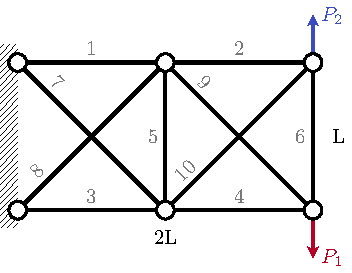
\includegraphics{figures/04_TTO_improvements/18_10_bar_multi_BC/10_bar_BC_multi.pdf}
    \caption{Ground structure of the ten-bar truss with two applied load cases $P_1$ and $P_2$.}
    \label{fig:04_10-bar-bcs-multi}
\end{figure}

\begin{figure*}
    \centering
    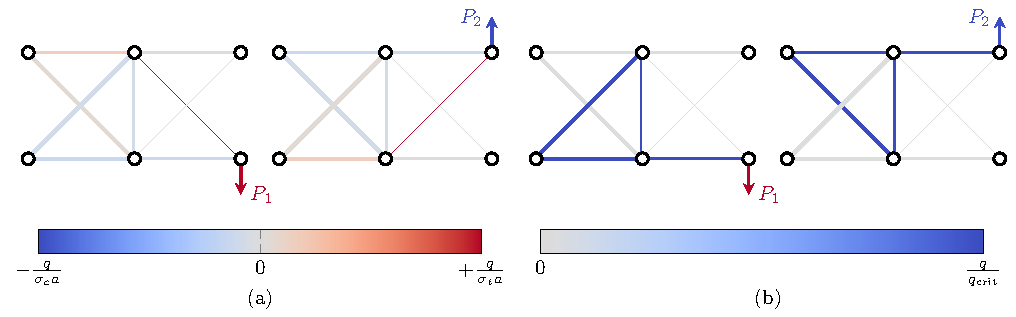
\includegraphics[width=\linewidth]{figures/04_TTO_improvements/19_10_bar_multi_opt/10_bar_multi_opt.pdf}
     \caption{Maximum stress constraint value (left) and buckling constraint value (right) plotted on the optimized design of the multiple load cases ten-bar truss.}
    \label{fig:04_10-bar-bcs-multi-opt}
\end{figure*}

In agreement with previous results, the proposed 2S-5R strategy reduces simultaneously the volume and the dispersion of the solutions. Interestingly, the mean value $\overline{V}$ of the 2S-0R algorithm is \qty{1.3}{\%} lower with respect to 2S-5R, a fact never observed before. This is due to the 2S-0R algorithm occasionally converging to a heavier solution in the \gls{slp} phase that results in a lighter solution once optimized by the \gls{nlp}, suggesting that the lightest \gls{slp} configuration does not always correspond to the lightest \gls{nlp} design. However, as the difference between the two solutions is low (\qty{3.9}{\%}), the 2S-5R algorithm is still preferred thanks to its higher solution consistency (the dispersion $\sigma$ of 2S-5R is \qty{71}{\%} lower than the dispersion $\sigma$ of 2S-0R).

We now analyze the lightest solution with a final volume of $V=134279.32$. The optimized design obtained is symmetric. This is consistent with Conjecture 4 made by Rozvany \sidecite{rozvany_symmetry_2011}, according to which if the boundary conditions and the ground structure are symmetric, and two alternate load conditions are mirror images of each other with respect to the symmetry axis, then at least one globally optimal topology is symmetric. This conjecture has been confirmed in \sidecite{guo_confirmation_2014} in the case of symmetric convex optimization problems. It is interesting to note that the Conjecture still holds for this specific example even if problem \ref{eq:04_optim_complete} is non-linear and non-convex. In \tabref{tab:04_10_multi_opt_comp} we list the cross-sectional area of the members for the two steps of the proposed solving optimization strategy. The \gls{nlp} optimized structure presents a volume $V=134279.32$, a \qty{35.15}{\%} increase compared to the predicted volume of the \gls{slp} step of $V=99084.93$. Incorporating kinematic constraints to achieve a solution that adheres to elasticity requirements significantly impacts the volume of the optimized solution. The design for the two different load cases $P_1$ and $P_2$ is shown in \figref{fig:04_10-bar-bcs-multi-opt}, where a side-by-side plot of the maximum stress and buckling constraints is presented. In this example, the bars are constrained by either the buckling or the stress of one of the two load cases. The detailed value of the design variables of the solution is given in \tabref{tab:04_10_multi_opt}, while the iteration history curves of the optimization can be found in \figref{fig:04_c1}.

\begin{table}
\small
\centering
\begin{tabular}{c S S S[retain-explicit-plus, table-format=3.2]} % Siunitx package special format
\toprule
\textbf{Bar} & {\textbf{SLP step} \eqrefnotext{eq:04_optim_no_constr}} & {\textbf{NLP step} \eqrefnotext{eq:04_optim_complete}} & \textbf{Difference} \\ \midrule
$a_1$        & 57.296       & 47.987       & \qty{-16.24}{\percent}                    \\
$a_2$        & 40.408       & 40.621       & \qty{+0.05}{\percent}                  \\
$a_3$        & 57.296       & 47.987       & \qty{-16.24}{\percent}                     \\
$a_4$        & 40.408       & 40.621       & \qty{+0.05}{\percent}                     \\
$a_5$        & 40.193       & 25.547       & \qty{-36.43}{\percent}                     \\
$a_6$        & 0.052        & 0.000        & \textemdash                     \\
$a_7$        & 6.997        & 53.115       & \qty{+659.11}{\percent}                     \\
$a_8$        & 6.997        & 53.115       & \qty{+659.11}{\percent}                     \\
$a_9$        & 6.997        & 7.071       & \qty{+0.01}{\percent}                    \\
$a_{10}$     & 6.997        & 7.071       & \qty{+0.01}{\percent}                     \\ \midrule
\multicolumn{1}{c}{V} & \multicolumn{1}{c}{99084.93} & \multicolumn{1}{c}{134279.32} & \qty{+35.51}{\percent}                 \\  
\bottomrule
\end{tabular}
\caption{Comparison of the results of the \gls{slp} step and \gls{nlp} step for the multiple load cases ten-bar truss.}
\label{tab:04_10_multi_opt_comp}
\end{table}

In \figref{fig:04_c1} we provide the iteration history of the objective function and the constraint violation for the \gls{slp} and the \gls{nlp} steps. The graphs on the left depict the evolution of volume during optimization in both the \gls{slp} and \gls{nlp} steps. Looking at the \gls{slp} step (red plot), we can see that the \gls{slp} reduces the volume and exhibits occasional "spikes," which correspond to the reinitialization heuristic calls. The gradual diminishment of these spikes throughout the optimization is due to the incorporation of the continuation scheme on the parameter $\phi_k$ of \eqref{eq:04_phi}. Turning our attention to the \gls{nlp} step, we observe that initially the volume is increased and then it descends again, stabilizing at a value that is higher than the one of the \gls{nlp} starting point. To elucidate this behavior, we refer to the graphs on the right, which present the history of constraint violations in the \gls{nlp} step. Notably, the starting point of the \gls{nlp} step always respects equilibrium $g_\text{eq}$ and kinematic compatibility $g_\text{comp}$, as displacements and forces are evaluated using \eqref{eq:04_truss_fem}. However, stress $g_\text{st,c}$ and $g_\text{st,t}$ and buckling constraints $g_\text{buck}$ are not initially respected, because the force field provided by the \gls{slp} does not account for the kinematic compatibility constraint. The \gls{nlp} optimizer then tries to reduce violations of buckling and stress while temporarily increasing its volume (a phase referred to as the "restoration phase" in the IPOPT algorithm). Ultimately, the optimizer converges to a volume that is slightly higher than what was predicted by the SLP. This aligns with the concept that, by disregarding kinematic compatibility in the \gls{slp} step, we have a lower-bound formulation for the volume.

\begin{table}
    \small
    \centering
    \sisetup{table-auto-round}
    \begin{tabular}{ccS[table-format=3.1]S[table-format=3.1]S[table-format=3.1]S[table-format=2.1]S[table-format=5.1]}
    \toprule
    \multicolumn{1}{c}{\textbf{($x_a$ $y_a$)}} &
      \multicolumn{1}{c}{\textbf{($x_b$ $y_b$)}} &
      \multicolumn{1}{c}{\textbf{$\ell$}} &
      \multicolumn{1}{c}{\textbf{$q_1$}} &
      \multicolumn{1}{c}{\textbf{$q_2$}} &
      \multicolumn{1}{c}{\textbf{a}} &
      \multicolumn{1}{c}{\textbf{V}} \\ \midrule
    (0 360)   & (360 360) & 360.00 & 160.45  & -139.55 & 47.99 & 17275.40 \\
    (360 360) & (720 360) & 360.00 & 0.00    & -100.00  & 40.62 & 14623.79 \\
    (0 0)     & (360 0)   & 360.00 & -139.55 & 160.45  & 47.99 & 17275.40 \\
    (360 0)   & (720 0)   & 360.00 & -100.00  & 0.00    & 40.62 & 14623.79 \\
    (360 0)   & (360 360) & 360.00 & -39.55	  & -39.55  & 25.55 & 9196.95  \\
    (360 0)   & (0 360)   & 509.12 & 55.93   & -85.49  & 53.12 & 27042.00 \\
    (0 0)     & (360 360) & 509.12 & -85.49  & 55.93   & 53.12 & 27042.00 \\
    (720 0)   & (360 360) & 509.12 & 141.42  & 0.00   & 7.07 & 3600.00  \\
    (360 0)   & (720 360) & 509.12 & 0.00   & 141.42  & 7.07 & 3600.00  \\ \midrule
    \multicolumn{1}{c}{} &
      \multicolumn{1}{c}{} &
      \multicolumn{1}{c}{} &
      \multicolumn{1}{c}{} &
      \multicolumn{1}{c}{} &
      \multicolumn{1}{c}{$\bm{V_{\text{tot}}}$} &
      \multicolumn{1}{c}{134279.32\textsuperscript{\emph{a}}} \\ \bottomrule
    \end{tabular}
    \\
    \footnotesize{\textsuperscript{\emph{a}}The total volume value is lower than the sum of the member volumes due to the one decimal places round-off.}
    
    \caption{Optimal values of the member forces, areas, and volumes of the members of the ten-bar truss with multiple load cases.}
    \label{tab:04_10_multi_opt}
    \end{table}

\begin{figure*}
    \hspace*{\fill}
    \subcaptionbox{}{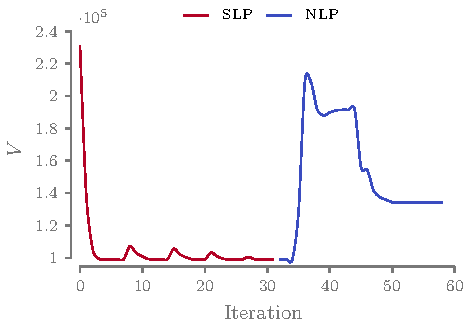
\includegraphics[width=0.49\linewidth]{figures/04_TTO_improvements/20_convergence_curves_ten_bar/10bar_hist.pdf}}
    \hfill
    \subcaptionbox{}{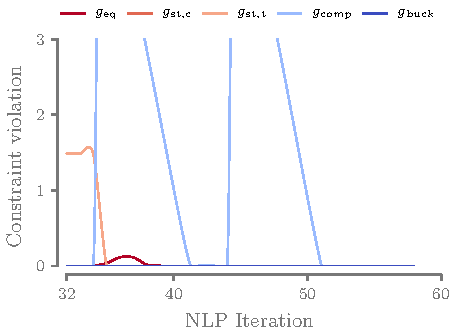
\includegraphics[width=0.49\linewidth]{figures/04_TTO_improvements/20_convergence_curves_ten_bar/10bar_constr.pdf}}
    \hspace*{\fill}
    \caption{Iteration history of the ten-bar truss with multiple load cases example solved with the 2S-5R algorithm; (a) objective function history for the \gls{slp} and \gls{nlp} step (b) constraint violation for the \gls{nlp} step.}
    \label{fig:04_c1}
\end{figure*}

\section{Conclusion}
In this chapter, we presented a structural optimization formulation that minimizes the mass of two- and three-dimensional truss structures subject to multiple load cases, maximum stress, topological buckling, and minimum slenderness constraints. The optimization is solved using an efficient two-step method and shows a reduced influence on the starting point thanks to the proposed reinitialization heuristic. Several numeric examples are presented using the proposed optimization algorithm. Optimized structures display designs with fewer active members compared to traditional optimization methods, leading to lower overall manufacturing complexity. Additionally, thanks to the computational efficiency of the proposed optimization strategy, we show how advanced mechanical constraints such as maximum stress, topological buckling, and kinematic compatibility constraints can be applied and solved on structures with thousands of candidates on a notebook computer.

However, some research questions still remain open. The manufacturing complexity is discussed here only as an outcome of the optimization strategy, but a direct way to impose manufacturing constraints (maximum numbers of bars converging to a single node, minimum section, imposed periodicity of the structure) during the optimization would be beneficial. For that reason, in the next chapters, we study the mechanical behavior of modular structures, exploring the trade-off between mechanical performance and manufacturing complexity.